\documentclass[twocolumn,twocolappendix,trackchanges]{aastex63}
\usepackage{amsmath}
\newcommand{\code}[1]{\texttt{#1}}
\newcommand{\mesa}{\code{MESA}}
\newcommand{\MESA}{\code{MESA}}
\renewcommand{\labelitemii}{$\bullet$}
\newcommand{\kms}{{\mathrm{km\ s^{-1}}}}
\newcommand{\Msun}{{\mathrm{M}_\odot}}
\newcommand{\kev}{\mathrm{keV}}
\newcommand{\gk}{\ensuremath{\,\rm{GK}}}
\usepackage{CJK}
\DeclareRobustCommand{\Eqref}[1]{Eq.~\ref{#1}}
\DeclareRobustCommand{\Figref}[1]{Fig.~\ref{#1}}
\DeclareRobustCommand{\Tabref}[1]{Tab.~\ref{#1}}
\DeclareRobustCommand{\Secref}[1]{Sec.~\ref{#1}}
\newcommand{\zoph}{$\zeta$ Oph}

\newcommand{\todo}[1]{{\large $\blacksquare$~\textbf{\color{red}[#1]}}~$\blacksquare$}

\defcitealias{villamariz:05}{VH05}


\begin{document}

\graphicspath{{./figures/}}


\title{Testing models of accreting stars in
  massive binaries on $\zeta$ Ophiuchi}
\author[0000-0002-6718-9472]{M.~Renzo}
\affiliation{Department of Physics, Columbia University, New York, NY 10027, USA}
\affiliation{Center for Computational Astrophysics, Flatiron Institute, New York, NY 10010, USA}

\author[0000-0002-6960-6911]{Y.~G\"otberg}
\affiliation{The Observatories of the Carnegie Institution for Science, 813 Santa Barbara Street, Pasadena, CA 91101, USA}


\begin{abstract}
  Most massive stars are born in binary systems close enough
  for mass-transfer episodes. These modify the appearance, internal
  structure, and future evolution of both stars. However,
  self-consistent models of the accretors are rare.  The nearest
  O-type star to Earth, $\zeta$ Ophiuchi, has long been
  proposed to have accreted mass from a former companion, before being
  ejected at the time of the companion's supernova
  explosion. Therefore, this star provides an ideal test bed for
  models of accretors in binaries. We use % the open-source stellar
  % evolution code
  \texttt{MESA} to model the evolution a massive binary
  ($M_1\gtrsim 20\,M_\odot\geq M_2$) evolving through a stable mass
  transfer after the donor's main sequence (case B, initial period 100\,days). Adopting common
  assumptions for the treatment of rotation, chemical mixing, and mass
  transfer efficiency, our models of the accreting star reproduce
  reasonably well the kinematic, spectroscopic, and photometric
  properties of $\zeta$ Ophiuchi. We compare the internal structure and evolution
  of our accretor to fast-rotating single stars, and find that the
  late and extreme spin up by binary interactions yields, at the end of
  the main sequence, a faster-spinning core in the accretor than in
  rotating single stars. Our models demonstrate the impact of mass
  accretion on the secondary star in a binary, with possible implications
  for its further evolution (either in a binary or as single stars),
  the final collapse, and the resulting spins of the compact object
  formed.
\end{abstract}

\vspace*{-10pt}
\keywords{stars: individual: $\zeta$ Ophiuchi  -- stars: massive --
  stars: binaries} %% check keywords exist

\section{Introduction}
\label{sec:intro}

The overwhelming majority of massive stars is born in multiple systems
\citep[e.g.,][]{mason:09, almeida:17}, and a large fraction will
exchange mass or merge with a companion in their lifetime
\citep[e.g.,][]{sana:12}. The most common type of interaction is a
stable mass transfer through Roche Lobe overflow (RLOF) after the end of the donor's main sequence (case
B, \citealt{kippenhahn:67}).  Many
studies %\todo{more refs. from other groups}
have focused on the dramatic impact these interactions have on the
donor star \citep[e.g.,][]{morton:60, yoon:17, gotberg:17, gotberg:18, laplace:20,
  laplace:21, blagorodnova:21}. Often the binary companion is treated as a point mass.

However, binary interactions have a crucial impact on the initially
less massive star too: during mass transfer, these are expected to
accrete mass, spin up to critical rotation
\citep[e.g.,][]{packet:81}, and possibly be polluted by
CNO-processed material from the inner core of the donor star
\citep[e.g.,][]{blaauw:93}. The growth of
the convective core due to the increased mass leads to
``rejuvenation'' of the accretor \citep[e.g.,][]{neo:77, schneider:16}.

Understanding the evolution of accretors in massive binaries has wider
and crucial implications for stellar populations, electromagnetic
transient observations, and gravitational-wave progenitors. Accretors
(and mergers) can appear as blue stragglers \citep[e.g.,][]{chen:09, chen:10} and thus impact cluster
populations and their age estimates and main sequence morphology
\citep[e.g.,][]{pols_marinus:94, wang:20}. The post-mass-transfer high
rotation rate might be the dominant explanation for the origin of
massive stars showing emission lines \citep[e.g.,][]{bodensteiner:20,
  vinciguerra:20}. Moreover, the majority of massive binaries will be
disrupted by the first supernova ejecting the companion
\citep[``binary SN scenario'', ][]{blaauw:61, dedonder:97,
  eldridge:11, boubert:18, renzo:19walk, evans:20}. Therefore,
populations of field massive stars contain presently single O-type
stars that accreted mass earlier on. A small fraction would be
sufficiently fast to become runaway stars, but the majority of these will be too
slow to stand out in astrometric surveys. Assuming a constant star
formation history, \cite{renzo:19walk} estimated that
$10.1^{+4.6}_{-8.6}\%$ of O-type stars could be `accretors released
after a SN. % -- where the errors span
% a range of parameter variations.


From the transients perspective, massive accretor stars are also
important: \cite{zapartas:19} showed that $14_{-11}^{+4}\%$ of
hydrogen-rich (type II) SNe might come from these progenitors after
being ejected from a binary. The fact that they accreted mass before
exploding can influence their helium (He) core mass and thus the
explosion properties and the inferred progenitors
\citep{zapartas:21}. The high post-mass transfer rotation rate of
accretor stars in binaries might have implications for the formation
of long gamma-ray burst progenitors \citep{cantiello:07}.

Finally, the majority of isolated binary evolutionary scenarios for
gravitational-wave progenitors include a common-envelope
phase. This is initiated by the originally less massive accretor,
after the formation of the first compact object
\citep[e.g.,][]{belczynski:16nat, tauris:17,
  broekgaarden:21}. Therefore, it is possible that accretion of mass
before the formation of the first compact object could modify the
internal structure of the star that will initiate the common-envelope
phase \citep[e.g.,][]{law-smith:20, klencki:21}. Specifically, the
rotation rate, chemical composition, and innermost structure of the
envelope (because of rejuvenation) might differ from a normal single
star.

Despite their importance, accretor stars in binaries have so far
received much less attention than the donor stars, with the pioneering
studies of \cite{ulrich:76, hellings:83, hellings:84}, and
\cite{braun:95} as notable exceptions. Large grids of accretor models
are lacking, most of the studies focus on lower mass systems
(e.g., \citealt{vanrensbergen:06, vanrensbergen:11}, but see also
\citealt{wang:20}) and only few sparse massive models exist
\citep[e.g.,][]{cantiello:07}. This is because of the difficulty of
modeling accretor stars, which requires following in detail the coupled
evolution of two rotating stars exchanging mass. Moreover, the
admittedly large number of free parameters involved in the modeling of
each individual star and their interactions makes robust predictions
challenging to obtain. We emphasize that rapid population synthesis
calculations typically cannot include the effects of binary mass
transfer on the internal structure of the stars, and rely on the
implicit assumption that the accretor is sufficiently well described
by a (possibly fast-rotating) single star model.

Here, we argue that the nearest O-type star to
Earth, $\zeta$ Ophiuchi\footnote{also known as HD\,149\,757.} (\zoph)
provides a unique opportunity to constrain these models.
\zoph\ has a distance from Earth of $107\pm4$\,pc \citep[][and
references therein]{neuhauser:20}, and a spectral type O9.5{\rm IVnn}
\citep{sota:14}. It occasionally shows emission lines, making it an Oe
star \citep{walker:79, vink:09}. Its surface rotation
rate is extremely large, with most estimates of the projected
rotational velocity from optical spectra exceeding
$v\sin(i)\gtrsim 400\,\kms$ \citep[corresponding to the ``nn'' in the
spectral type, e.g.,][]{zehe:18}. Using optical
interferometry, \cite{gordon:18} were able to measure its centrifugal
distorsion, suggesting close-to-breakup rotation.

\zoph\ was originally
identified as a runaway because of its large proper motion by
\cite{blaauw:52}. Unfortunately, the \emph{Gaia} data for this object
are not of sufficient quality\footnote{The renormalized unit weighted
  error (RUWE) of this star in Gaia EDR3 is 4.48.} to improve previous astrometric results,
but estimates of the peculiar velocity range in $30-50\,\kms$
\citep[e.g.,][]{zehe:18, neuhauser:20}. The large velocity with
respect the surrounding interstellar material is also confirmed by the
presence of a prominent bow-shock \citep[e.g.,][]{bodensteiner:18}.

Because of its young apparent age, extremely fast rotation, and nitrogen
(N) and He rich surface \citep[e.g.,][]{herrero:92, blaauw:93,
  villamariz:05, marcolino:09}, \zoph\ is a prime candidate for the
binary SN scenario \citep{blaauw:93}. Many studies have suggested
\zoph\ might have accreted mass from a companion before acquiring its
large velocity, both from spectroscopic and kinematic considerations
\citep[e.g.,][]{blaauw:93, hoogerwerf:00, hoogerwerf:01, tetzlaff:10,
  neuhauser:20} and using stellar modeling arguments
\citep[e.g.,][]{vanrensbergen:96}. Recently, \cite{neuhauser:20}
suggested that $1.78\pm0.21$\,Myr ago a supernova in
Upper-Centaurus-Lupus produced the pulsar PSR B1706-16, ejected \zoph,
and also injected the short-lived radioactive isotope
$^{60}\mathrm{Fe}$ on Earth. This argues strongly for a successful
supernova explosion of the companion with a large $\sim 250\,\kms$ natal
kick, which in most cases would be sufficient to disrupt the binary
\citep[e.g.,][]{tauris:15, renzo:19walk, evans:20}.

Although the nature of \zoph\ as a binary product is well established,
because of its observed large surface rotation rate, previous attempts
to model it rely purely on rotational mixing to explain the surface
composition \cite[e.g.,][]{maeder:00}. Even the binary models of
\cite{vanrensbergen:96} assumed spin-up due to mass accretion to drive
rotational mixing from the interior of the accreting star (see also
\citealt{cantiello:07}). However, \cite{villamariz:05} (hereafter,
\citetalias{villamariz:05}) were unable to find good fit for the
stellar spectra using the rotating models from \cite{meynet:00, meynet:03}.

This may not be surprising: rotational mixing has lower efficiency for
metal-rich and relatively low mass stars because of the increased
importance of mean molecular weight gradients and longer thermal
timescales compared to more massive stars \citep[e.g.,][]{yoon:06,
  perna:14}. The parent association has a metallicity
$Z=0.01\simeq Z_\odot$ \citep[based on asteroseismology
from][]{murphy:21}, and mass estimates for \zoph\ range from
$13-25\,M_\odot$, at the lower end of the range where efficient mixing
might bring He and CNO-processed material to the surface (chemically
homogeneous evolution, \citealt{maeder:00}).

Given the challenges in explaining the surface composition of \zoph\
with rotational mixing from the stellar interior and the strong
evidence for its past as a member of a binary system, this star offers
a unique opportunity to constrain the evolution of accreting stars in
massive binary systems. Here, we present self-consistent binary evolution models for
$\zeta$ Oph computing simultaneously the coupled evolution of
\emph{both} donor and accretor star and their orbit. After presenting
our \texttt{MESA} setup in \Secref{sec:methods}, we show our best model which
reproduces the majority of the salient features of this star in
\Secref{sec:best_model}. %  In this model, the surface abundances of
% \zoph\ are explained by pollution from the former companion, rather
% than upward mixing from the interior of \zoph\ itself.
We discuss the
sensitivity of our results to the admittedly many free parameters
required for this kind of computations in
\Secref{sec:discussion}. Finally, we conclude in
\Secref{sec:conclusions}.



\section{Modeling massive binaries with \texttt{MESA}}
\label{sec:methods}

Modeling the evolution of massive binaries
($M_1\gtrsim 20\,M_\odot \geq M_2$) is challenging because of the
intricate role of several notoriously difficult stellar physics
ingredients (differential rotation, mixing, high mass-loss rates,
accretion, etc.). Here we follow self-consistently the coupled
evolution of two massive stars in a binary system using \texttt{MESA}
(version 15140, \citealt{paxton:11, paxton:13, paxton:15, paxton:18, paxton:19}). Our choice of input parameters and our numerical
results are available at \url{10.5281/zenodo.4701565}. We discuss here only the main
relevant physical parameters and describe tests changing some of the
fiducial values in \Secref{sec:discussion}. Appendix~\ref{sec:software} gives
more details on our choice of input physics, and
appendix~\ref{sec:res_tests} discuss the numerical resolution in space and time.

We adopt the Ledoux criterion to determine convective stability and a
mixing length parameter of $1.5$. We include semiconvection and
thermohaline mixing following \cite{langer:83} and
\cite{kippenhahn:80}, respectively, each with efficiency $1.0$. We use the exponential core overshooting from \cite{herwig:00}
with free parameters\footnote{See Eq.~2 in \cite{paxton:11}.} $(f, f_0)=(4.25\times10^{-2}, 10^{-3})$
\citep{claret:17} which broadly reproduce the width of the main
sequence from \cite{brott:11}. We also use the local implicit
enhancement of the convective flux in superadiabatic regions
(\texttt{MLT--}) introduced in \texttt{MESA}
15140.

We treat rotation in the ``shellular'' approximation, that is we assume constant
rotational frequency $\omega$ along isobaric surfaces. Furthermore, we assume
tidal synchronization at the beginning of our runs. For our fiducial
period choice ($P=100$\,days), this effectively means the stars
in our binary are initially slow rotators: the surface averaged
rotational velocity is $\lesssim3\,\kms$ for both stars. Our models include a
diffusive approximation for Eddington-Sweet circulations
\citep{sweet:50}, which dominates the chemical mixing due to
rotation. We also include the secular and dynamical shear
instabilities, and the Goldreich-Schubert-Fricke instability, but
these remain subdominant throughout the evolution of our models.  We assume a
Spruit-Tayler dynamo for the transport of angular momentum
\citep{spruit:02}, and chose the same free parameters as
\cite{heger:00}. This also includes the rotational enhancement of wind
mass loss as in \cite{langer:98}.

We assume a fiducial metallicity of $Z=0.01$ informed by the
present-day $Z$ of the parent cluster \citep{murphy:21}, and assume
scaling of the relative element abundances with the solar abundances
of \cite{grevesse:98}. We include wind mass loss with the
\cite{vink:00,vink:01} hot wind, and \cite{dejager:88} for effective
temperature $T_\mathrm{eff}<10^{4.2}$\,K, both with a scaling
factor of 1. Nominally, this means our wind mass-loss rate post-mass
transfer is overestimated by almost a factor of 100 compared to
observations \citep[weak wind problem, see][]{marcolino:09}.  However,
\cite{lucy:12} and \cite{lagae:21} proposed that the temperature
structure of the winds of low-luminosity O-type stars might affect the
spectral lines and cause an empirical underestimate of the mass-loss
rate.

Both stars are evolved simultaneously on the same timesteps until
after the donor detaches from its Roche lobe. We follow \cite{kolb:90}
to calculate with an implicit scheme the mass transfer rate from optically thick layers of the
donor star during Roche lobe overflow (RLOF). Moreover, we assume that
the specific angular momentum and entropy of the transferred layers
match the surface, while the chemical composition is
set by the stratification of the donor star. Mass transfer is
conservative until the accretor reaches critical rotation, after which
rotationally-enhanced mass loss governs the mass transfer efficiency.

% To define RLOF detachment, we take advantage of the fact that we focus
% here on case B interactions among massive stars.
After losing their envelope, massive donors are not expected to expand
to hundreds of $R_\odot$ during He-shell burning at the metallicity we
consider \citep[e.g.,][]{laplace:20}. Thus, we stop evolving a binary
system when the donor's surface He mass fraction is larger than 0.35
-- indicating that a significant amount of envelope has been lost or
transferred, and the radius is smaller than both the Roche radius and
the terminal-age main sequence radius (TAMS, defined as when the
central mass fraction of H drops below $10^4$). From here onwards, % At this point in time,
% we save a model for the accreting star, and continue its evolution
% as
we continue the evolution of the accretor as a single star until its TAMS
with the same setup.

We discuss some parameter variations for the physics of each star, the
initial conditions, and the binary interactions in \Secref{sec:discussion}.

\section{Massive binary evolution naturally explains $\zeta$
  Ophiuchi's properties}
\label{sec:best_model}

\begin{figure}[bp]
  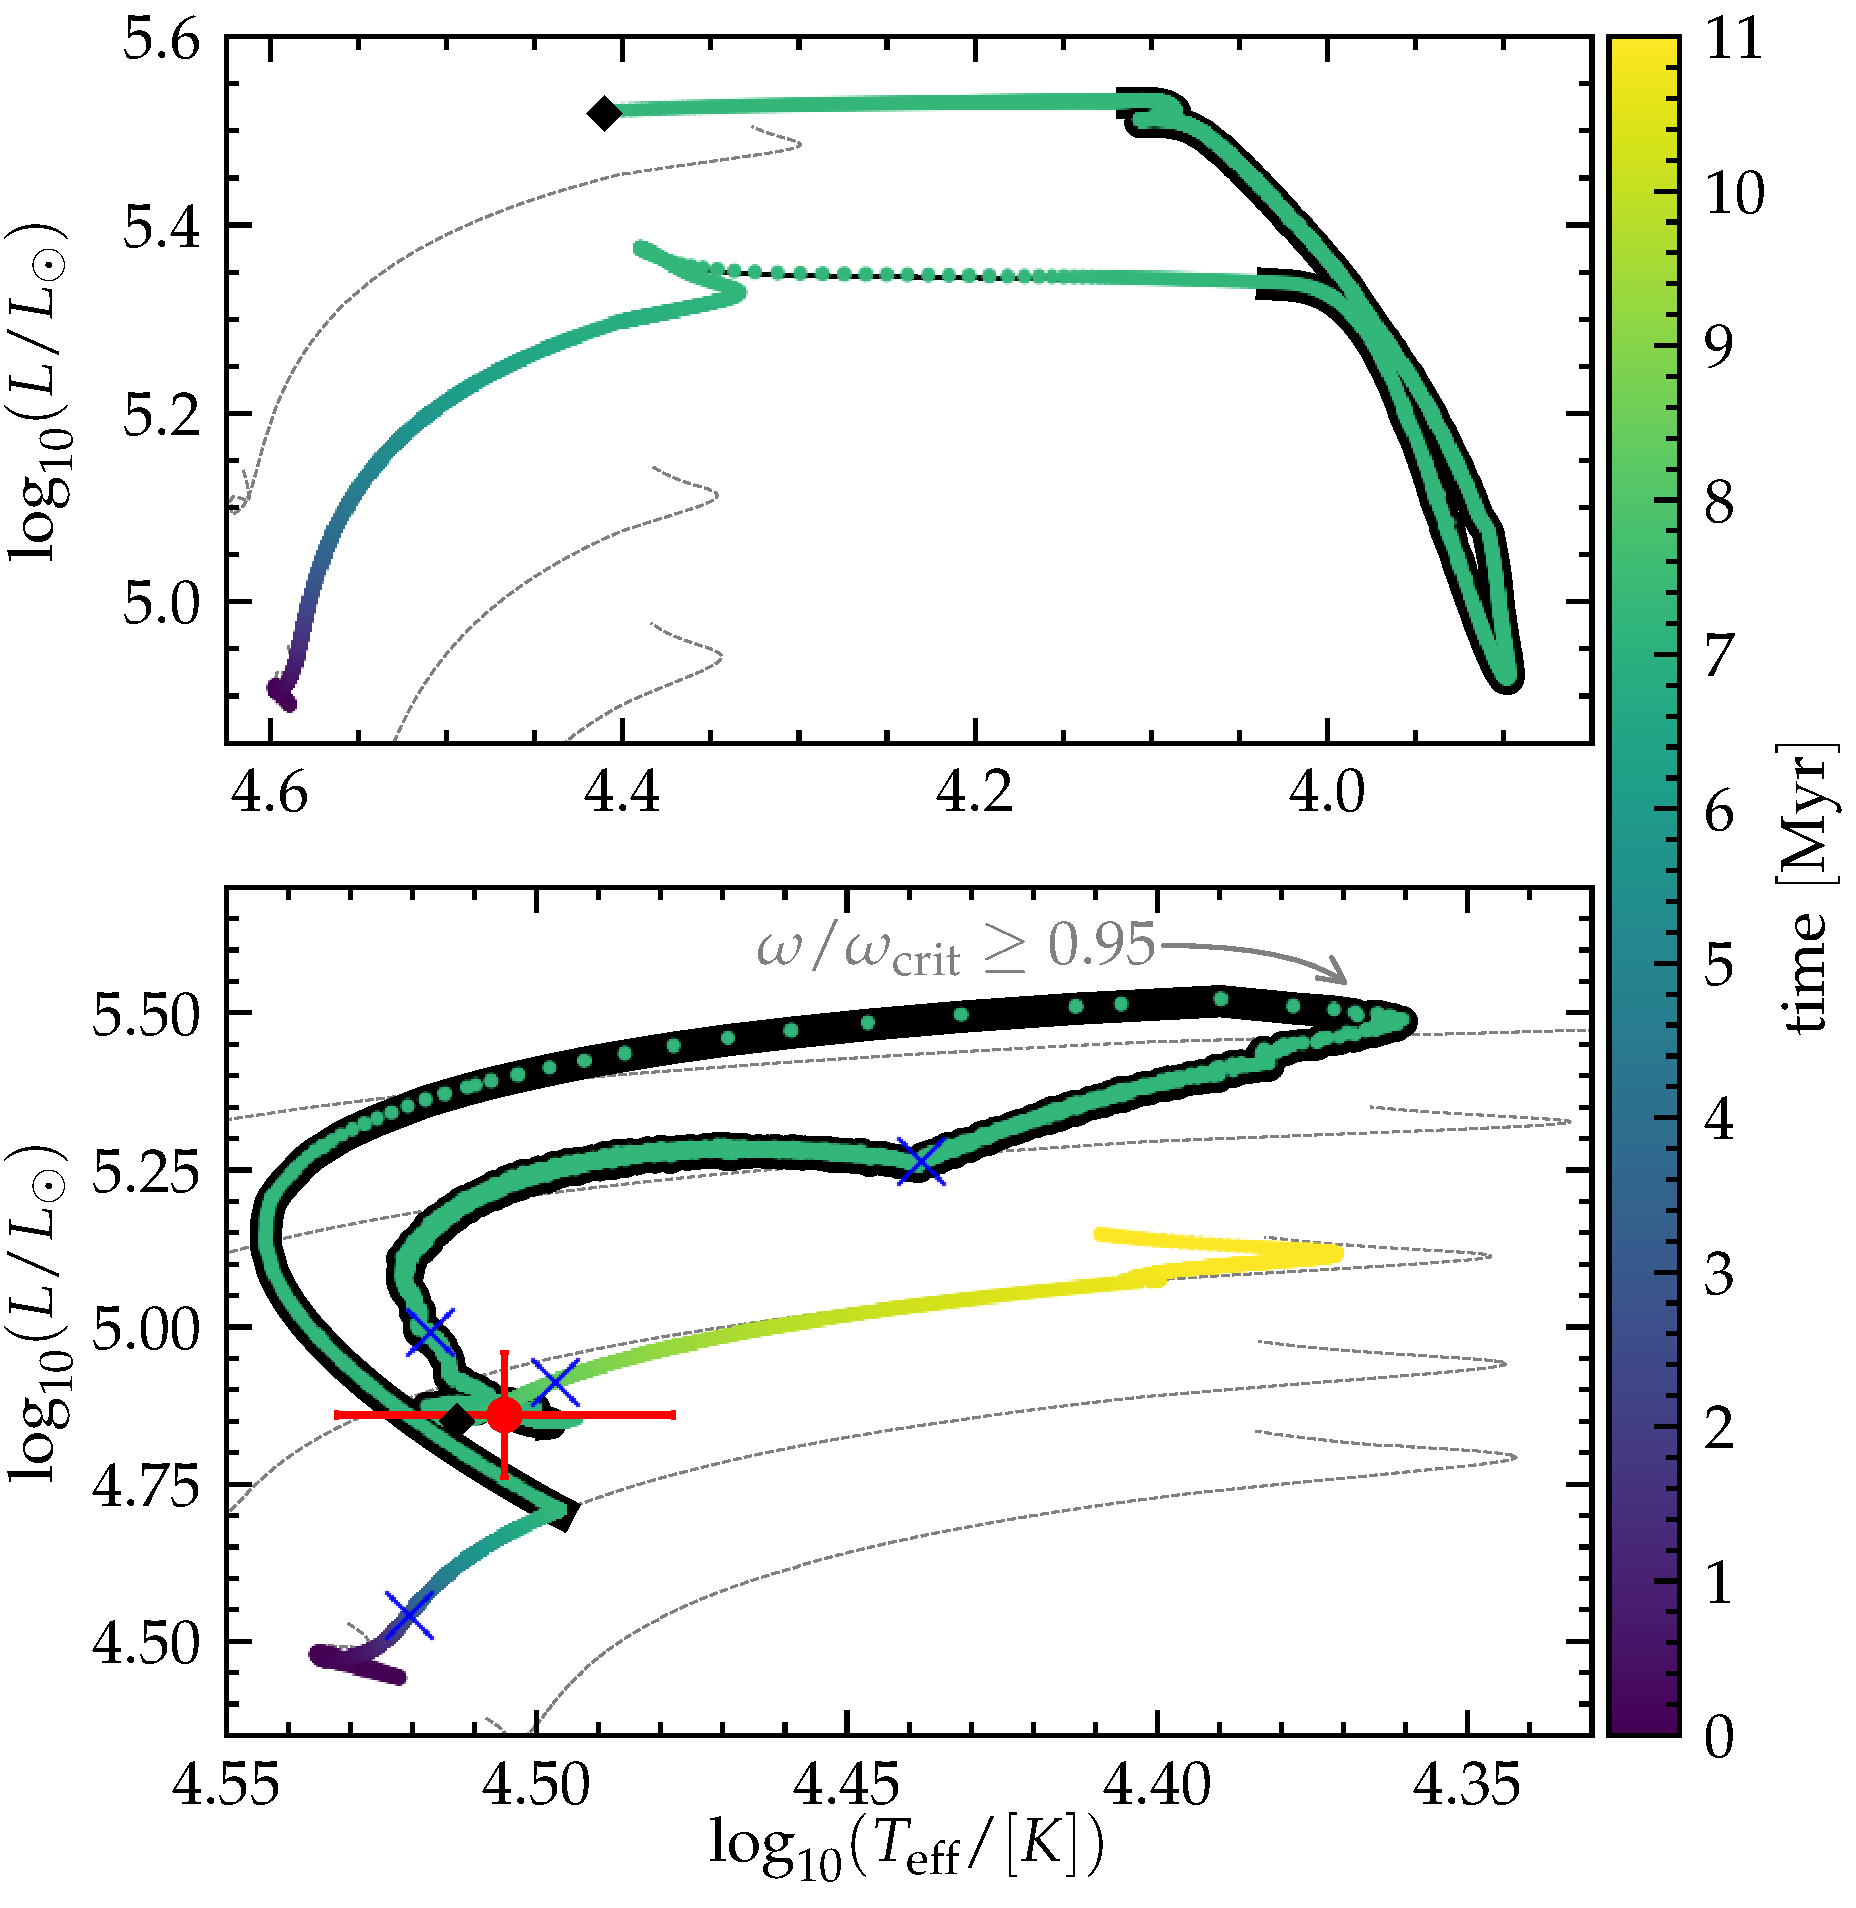
\includegraphics[width=0.5\textwidth]{HRD_both}
  \caption{HRD for the donor star (top) and accretor star (bottom) of
    the progenitor binary of \zoph. Each point is separated by 50
    years of evolution. The colors represent the
    stellar age, the red datapoint shows the position of \zoph\
    according to \citetalias{villamariz:05}, thin blue crosses mark the
    position of the profiles shown in \Figref{fig:D_mix}, and the black diamonds mark the
    position at the end of the binary run. We continue the accretor
    evolution as a single star from there until core H depletion,
    hence the bottom panel shows a longer time. We emphasize the different
    scales on the two panels. The thin gray dashed line show the main
    sequence evolution of non-rotating single stars of 15, 17, 25, and
    30\,$M_\odot$ at $Z=0.01$ for comparison.}
  \label{fig:HRD_both}
\end{figure}


We describe here the evolution of a binary system where the accretor
star can broadly reproduce all the observed features of \zoph. We
assume initial masses $M_1=25\,M_\odot$, $M_2=17\,M_\odot$ and initial
period $P=100$\,days with a metallicity of $Z=0.01$.

\Figref{fig:HRD_both} shows the Hertzsprung-Russell diagrams (HRD) of
both stars. After
$\sim$$7.24$\,Myr, the donor star (top panel) evolves off the main sequence and
$\sim8400$\,years later, when the donor's effective temperature reaches about $T_\mathrm{eff}\simeq
10^4$\,K, mass transfer starts. This results in a stable case B RLOF. We refer to \cite{gotberg:17, klencki:20, laplace:21, blagorodnova:21} and references therein for a detailed description of the evolution of massive donor stars in binaries. Although our models are more massive, the qualitative behavior of the donor star is similar. Minor differences might arise because of the complex behavior of the intermediate convective zone above the H-burning shell \citep[][]{klencki:21}, and its interplay with the mass transfer.

At the onset of RLOF, the accretor star (bottom panel of \Figref{fig:HRD_both}) is still on the main sequence with
$T_\mathrm{eff}\simeq10^{4.5}$\,K. Because of accretion, it is pushed out of thermal equilibrium and quickly becomes over-luminous to radiate away the excess internal energy and reaches $L\simeq10^{5.5}\,L_\odot\gg
L_\mathrm{nuc}\simeq
q10^{5.1}\,L_\odot$, with
$L_\mathrm{nuc}$ the total energy released per unit time by nuclear burning.

The radius of the accretor increases dramatically from
$\sim7.5\,R_\odot$ to $\sim35\,R_\odot$, and only once the accretor
reaches critical rotation (roughly at the lowest $T_\mathrm{eff}$ in
the bottom panel of \Figref{fig:HRD_both}), the star begins
contracting and its $T_\mathrm{eff}$ increases. At
$T_\mathrm{eff}\simeq 10^{4.43}$\,K the material transferred from the
companion star becomes progressively more He-rich and CNO-processed,
causing a ``v-shaped'' feature in the evolutionary track. This
indicates that the partially processed outer layers of the donor's
core are uncovered by mass
transfer. % after the convective core recession in
% mass during the main sequence.
This late mass transfer puts material at high mean molecular weight
$\mu$ on top of the primordial envelope of the accretor, modifying the
morphology of the evolutionary track. Thermohaline mixing starts in
the outer layers of the accreting star, and, together with rotational
mixing, it progressively dilutes the surface He and N mass fractions
and causes noisy features on the HR diagram
\citep[e.g.,][]{cantiello:07}. The (standard) algorithmic choices in
modelling mixing and rotation might impact the morphology of the
accretor's evolutionary track during RLOF. The entire duration of RLOF
is only about $10^4$\,years, and therefore unlikely to be observable
to probe directly the accuracy of our treatment of mixing. We expand
on the mixing processes inside the accretor in \Secref{sec:mixing}.

We evolve the binary system until the black diamonds in
\Figref{fig:HRD_both}, which occurs well after the donor detaches from
the Roche Lobe. At this point, the accretor is a H-rich fast-rotating
star of
$\sim$$20.1\,M_\odot$. Available mass estimates for the presently single \zoph\ are highly uncertain, but most include
$20\,M_\odot$ (e.g., \citealt{hoogerwerf:01}, \citetalias{villamariz:05}, \citealt{neuhauser:20}). The accretor's post-RLOF orbital velocity is
$v_2\simeq52\,\kms$. In the subsequent evolution, wind mass loss from both stars will result in  widening of the binary and slowing down of the accretor: we computed one binary model until the donor's He core burning, and at that point the accretor's orbital velocity has decreased to
$\sim$$40\,\kms$. Further decrease should be expected because of the
post-He core burning wind mass loss, likely dominated by the
(uncertain) mass-loss rate of the stripped donor star. Nevertheless,
the value we obtain is in broad agreement with estimates of the
observed runaway velocity of \zoph.

Accounting for both wind mass loss and the amount of mass transferred, at the end of RLOF the donor becomes a He star of
$\sim$$9.4\,M_\odot$, likely to contract further and appear as a
Wolf-Rayet star. It's surface H mass fraction is $\lesssim 0.2$ and
most of the H is likely to be removed by further wind mass loss
\citep[e.g.,][]{gotberg:17}.

From the black diamond onwards, we evolve the accretor as a single star with the same \texttt{MESA} setup until TAMS. The main-sequence track on which the accretor settles post-RLOF has a higher luminosity compared to the original track because of the accretion of mass, and it has also a slightly different slope due to the close-to-critical rotation and the accretion of partially nuclearly processed material (He- and N-rich) material.

The red errorbars in the bottom panel of \Figref{fig:HRD_both} mark the approximate position of \zoph\ based on the analysis of \citetalias{villamariz:05}. The color of the track in \Figref{fig:HRD_both} indicate that our accreting star spends about
$\sim$2\,Myr within the represented errorbars after the end of RLOF. Assuming the kinematic age of
$1.78\pm0.21$ \citep{neuhauser:20}, and estimating a remaining lifetime of the donor of
$\sim$0.5\,Myr, this gives the correct timescale for the binary SN scenario.

\begin{figure}[htbp]
  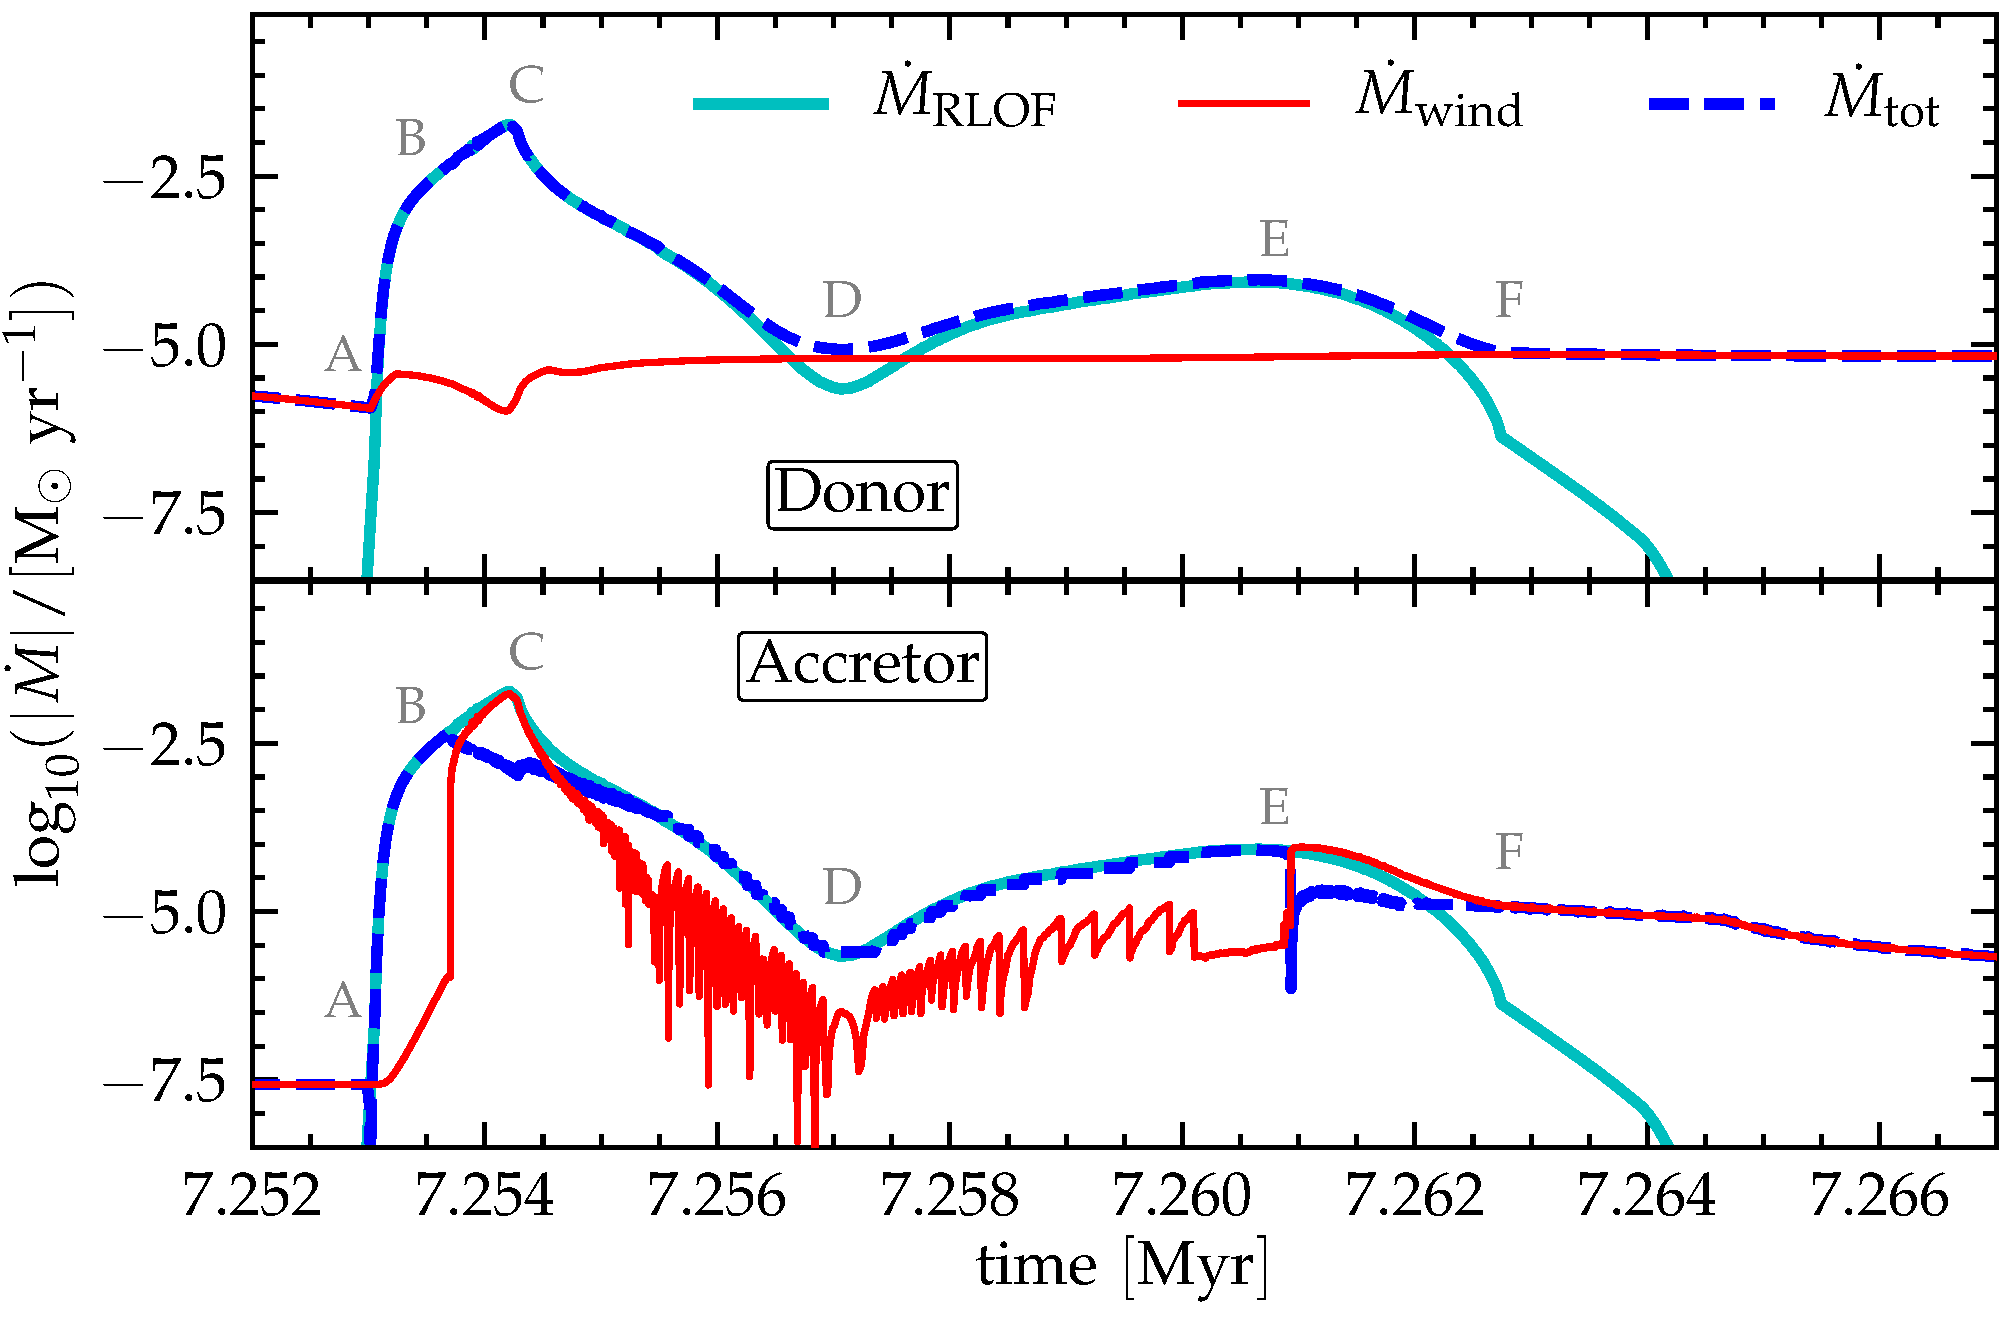
\includegraphics[width=0.5\textwidth]{MT}
  \caption{Mass transfer rates as a function of time during RLOF. The top (bottom) panel
    shows the donor (accretor) star. The cyan solid lines show the
    mass transfer rate between the two stars. The dashed blue lines
    show the actual change in the mass of the stars (due to the
    combination of wind, and accretion efficiency). The thin red
    lines show the wind mass loss rates. During RLOF the accretor
    reaches critical rotation, which leads to oscillations in the
    rotationally-enhahnced wind mass loss.}
  \label{fig:MT}
\end{figure}

\Figref{fig:MT} shows the rate of mass change for each star during
RLOF. The top panel focuses on the donor star which loses mass to RLOF
(cyan line) and wind mass loss (thin red line). The dashed blue lines
show their combination resulting in the actual rate of mass change of
the stars. The bottom panel shows instead the accreting star, which
grows in mass because of the mass transfer. At peak, the mass transfer
rates reaches very high values above
$10^{-2.5}\,M_\odot\ \mathrm{yr^{-1}}$ and taps into the optically
thick matter of the donor.

In the bottom panel, initially the mass transfer rate equals the rate
of change of mass of the accretor. This shows that initially the
accretion is (by construction) fully conservative. As the mass and
surface rotation rate of the accretor increase, the wind mass-loss
rate increases progressively by $\sim$5 orders of magnitude because of
the rotational enhancement \citep{langer:98}. The
rotationally-enhanced wind controls the accretion efficiency, and at
$\sim$$7.254$\,Myr the mass transfer becomes briefly non-conservative (where the red solid line and the cyan line overlap): the majority of the transferred mass is ejected away in a wind by the accretor. Consequently, the accretor can slightly spin down and starts contracting (cf.~\Figref{fig:HRD_both}). In the remaining evolution, the interplay between the wind mass loss rate, the spin-up due to accretion and the spin-down due to inward transport of angular momentum (see \Secref{sec:rot}) lead to the oscillations seen in the wind mass loss rate, but for most of the evolution accretion, albeit not-fully conservative, still occurs. This allows for CNO-processed material from the donor to reach the surface of the accretor during late stages of mass transfer.



% The wind mass loss (in red) controls the accretion efficiency and thus
% the difference between the actual rate of change in mass of the
% accretor (thick dashed blue) and the rate at which mass is being
% transferred. At peak, where the red and the cyan lines overlap, mass
% transfer becomes very non-conservative, but for most of the evolution
% the (rotationally enhanced) wind removes only a fraction of the
% accreted mass.

%  The interplay between the stellar radius and rotation
% causes the oscillations visible in the bottom panel, whose amplitude
% is generally lower than the RLOF mass transfer rate.



At the end of RLOF, the donor star briefly expands again
($T_\mathrm{eff}\simeq10^{4.1}$\,K, $L\simeq10^{5.5}\,L_\odot$). This
is due to the partial recombination of the now He-rich outer layers,
which causes a transient surface convection layer. This causes a
radial expansion of the outer convective layers and an increase in the
mass-transfer rate, despite at this point the donor is less massive
than the accretor and the binary is widening.  During this phase, the
mass transfer becomes fully non-conservative again (in the bottom
panel the wind and the mass accretion rate briefly become equal again
at $\sim7.261$\,Myr). We find this to be the culprit of the numerical
difficulties for massive mass-transferring binaries with older
\texttt{MESA} releases: although only a very small amount of mass is
involved, the onset of convection causes a large radius variation
which impacts the mass transfer rate.

\subsection{Mixing and composition}
\label{sec:mixing}

\begin{figure*}[htbp]
  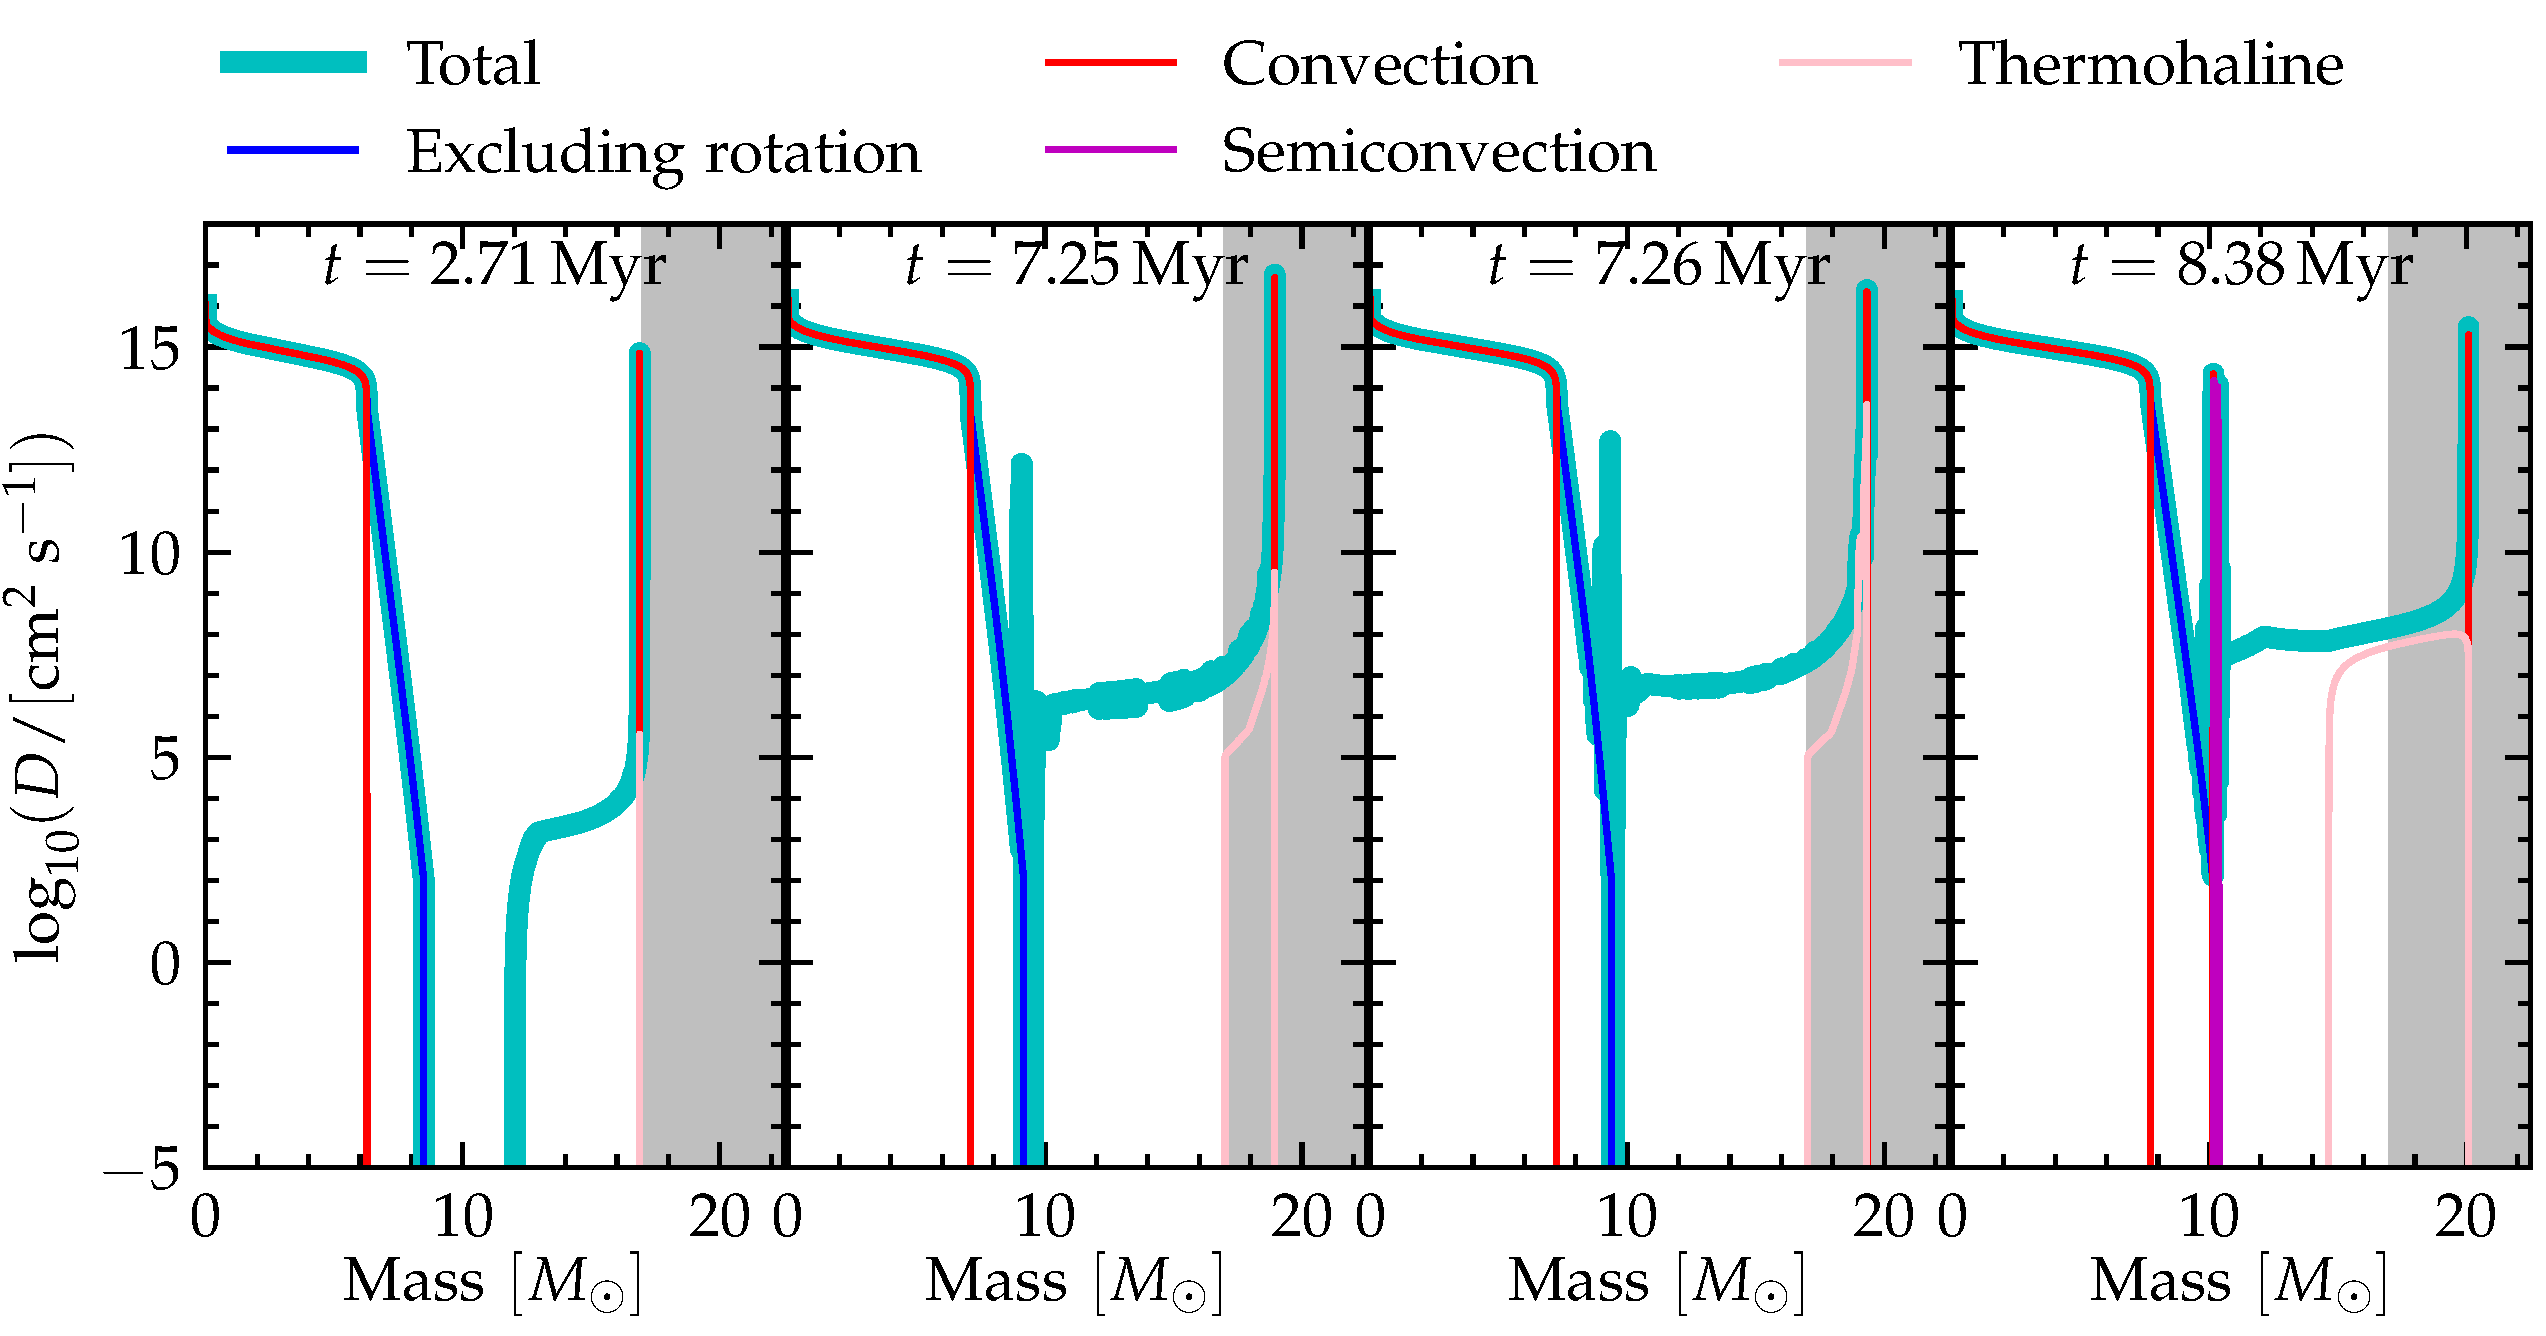
\includegraphics[width=\textwidth]{D_mix}
  \caption{Mixing diffusion coefficients in the accretor star. From
    left to right, each panel shows times during the main sequence
    (2.71\,Myr), right before the ``v-shaped'' feature during RLOF
    (7.25\,Myr), close to the end of RLOF (7.26\,Myr), and after mass
    transfer (8.38\,Myr) -- see the corresponding thin blue crosses in
    \Figref{fig:HRD_both}. The total diffusion coefficient (thick cyan
    line) is obtained as the sum of overshooting (thin blue line),
    convection (shown in red), thermohaline mixing (pink) and
    semiconvection (in purple), and rotational mixing -- which is
    largely dominated by Eddington-Sweet circulations. The gray area corresponds to mass
    accreted during
    RLOF.}
  \label{fig:D_mix}
\end{figure*}

\begin{figure*}[htbp]
  \centering
  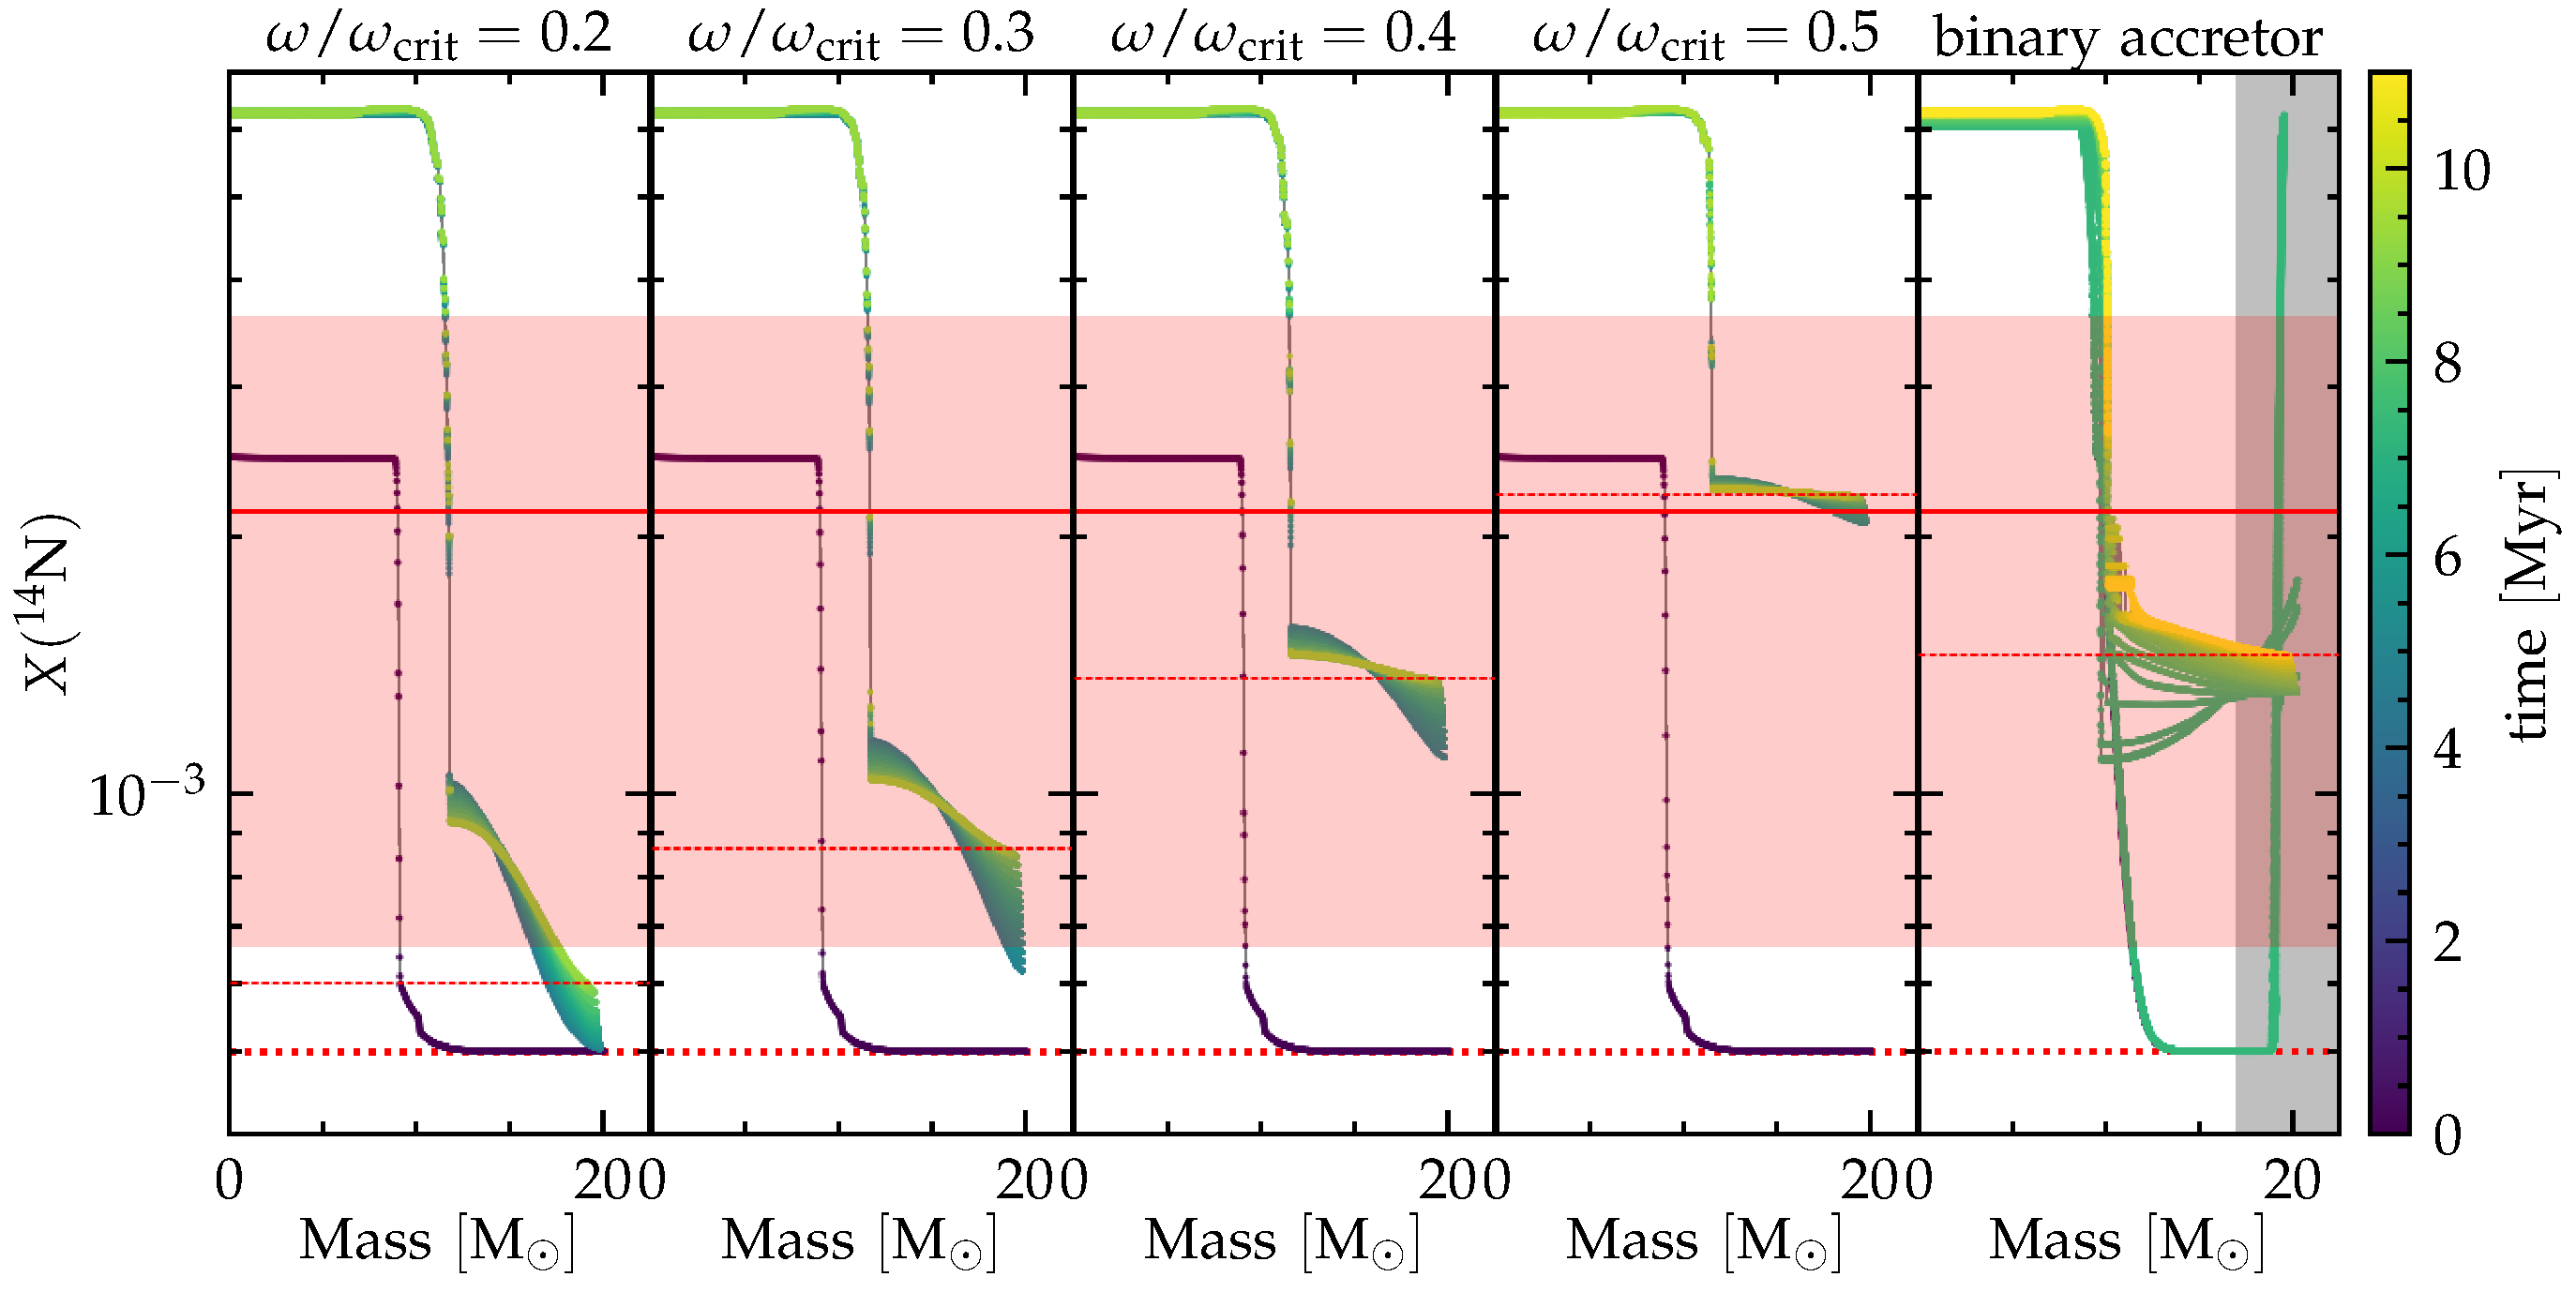
\includegraphics[width=\textwidth]{n14_struct_complete_zeta_ab}
  \caption{$^{14}\mathrm{N}$ mass fraction as a function of mass
    coordinate for $20\,M_\odot$ single star models with increasing
    $\omega/\omega_\mathrm{crit}$ at birth (first four panels), and
    for the accretor of our fiducial binary. The dotted thick red line
    marks the primordial value, the thin dashed red line marks the
    surface value at TAMS. In the last panel, the gray area highlights
    mass accreted during RLOF. The colors of each profile go from dark to
    light at TAMS, and selected profiles along the main sequence are
    shown. The solid red line and the shaded red region correspond to the
    mass fraction of $^{14}\mathrm{N}$ estimated by
    \citetalias{villamariz:05} assuming the surface mass fraction of H
    from \Tabref{tab:surf_prop}. The abundance of $^{14}\mathrm{N}$
    alone is not strongly constraining. \Figref{fig:composition_huge}
    shows a similar plot containing also $^{12}\mathrm{C}$ and $^{16}\mathrm{O}$.}
  \label{fig:n14}
\end{figure*}


\texttt{MESA} treats mixing in the diffusion approximation
\citep{paxton:11}.  To illustrate the dominant processes throughout
the accretor's evolution, we show in \Figref{fig:D_mix} the diffusion
coefficients for various mixing processes as a function of mass
coordinate at selected times. Each panel corresponds to one of the
thin blue crosses in the bottom panel of \Figref{fig:HRD_both}, and
the gray shaded areas highlight mass accreted during RLOF. The last
panel roughly represents the predicted internal structure of \zoph\ as
observed today.

In \Figref{fig:D_mix}, the thin red lines correspond to convection,
with the initial convective core of
$\sim$$6\,M_\odot$ clearly visible in the first panel. In all models, a tiny sub-surface convective region is also visible in the outermost layers (see e.g., \citealt{cantiello:21}).  The thin blue lines show the exponentially decreasing overshooting above the convective core. Purple and pink represent semiconvection and thermohaline mixing, respectively. Before mass transfer (left-most panel), only a small amount of sub-surface thermohaline mixing occurs, with a mass extent comparable or smaller to the sub-surface convective zone, and no semiconvection occurs. The thick cyan line corresponds to the total diffusion coefficient, obtained as the sum of the diffusion coefficients for each process modeled: where the cyan line is not overlapping with the others, rotational mixing (and more specifically Eddington-Sweet meridional circulation) is the dominant process.

During RLOF (second and third panel), the spin-up due to accretion causes an increase in the rotational mixing (see also \Secref{sec:rot}), and the accretion of nuclearly processed material progressively widens the thermohaline mixing region at the surface. Late during the mass transfer (third panel), thermohaline mixing dominates the outermost layers -- except within the sub-surface convective zone. Nevertheless, throughout most of the envelope, rotation does the lion's share of the mixing. Thermohaline mixing and Eddington-Sweet circulations together mix inwards and dilute the CNO-enriched material coming from the donor's surface.

At the same time, the increase in the accretor mass drives
rejuvenation \citep[e.g.,][]{schneider:16}. This can be seen as a
growth of the convective core from
$\sim$$6\,M_\odot$ to almost $\sim$$8\,M_\odot$, plus the
corresponding growth of the overshooting region. This mixes inward
H-rich material resulting in an elongation of the accretor's lifetime,
and at the same time mixes outward CNO-equilibrium matter, connecting
the N-rich core with the outer envelope polluted from the top.


    % this table was automatically generated using the table.ipynb in the repository associated to this manuscript
    \begin{table*}[hbpt]
    \centering
    \begin{tabular}{c|c|c|c|c|c|c|c|c}
    \hline\hline
    $M \ [M_\odot]$ & $R\ [R_\odot]$ & $\log_{10}(\omega / [\mathrm{s^{-1}}])$ & $v_\mathrm{rot} \ [\kms] $ & $X(^{1}\mathrm{H})$ & $X(^{4}\mathrm{He})$ & $X(^{12}\mathrm{C})$ & $X(^{14}\mathrm{N})$ & $X(^{16}\mathrm{O})$ \\
    \hline
    20.1 & 9.6 & -4.263 & 366.1 & 0.678010 & 0.312093 & 0.001344 & 0.001340 & 0.004148 \\
    \hline
    \end{tabular}
    \caption{Properties of the accretors shortly after the end of RLOF
    (last thin blue cross in \Figref{fig:HRD_both})}
    \label{tab:surf_prop}
    \end{table*}
    


\Tabref{tab:surf_prop} summarizes the surface properties of the
accretor star at the time shown in the last panel of
\Figref{fig:D_mix}, that is shortly after the RLOF phase, while the
model is still roughly at the observed position of \zoph.

Both the mass and radius agree reasonably well with the estimates from
\citetalias{villamariz:05} and previous studies, that is~$20\,M_\odot$ and
$8.3\pm1.5\,R_\odot$, respectively. Recently, optical interferometry
of \zoph\ suggested a polar radius of $7.5\,R_\odot$ and centrifugally
increased equatorial radius of $9.1\,R_\odot$ \citep{gordon:18}, also
in good agreement with our model.

The surface rotational velocity in
excess of $350\,\kms$ is also in the correct ballpark albeit possibly
on the low end. We discuss further rotation and angular momentum
transport in \Secref{sec:rot}.

We report the surface H mass
fraction\footnote{This is needed to convert mass fractions reported
  here into $\varepsilon(X)=12+\log_{10}(N_X/N_H)$, where $N_X$ and
  $N_H$ are the number fractions of species $X$ and H, respectively.},
lower than primordial because of the accretion of nuclearly processed
material, and the surface mass fraction of the most prominent species
$^4\mathrm{He}$, $^{12}\mathrm{C}$, $^{14}\mathrm{N}$,
$^{16}\mathrm{O}$.  Assuming our surface H mass fraction
$X(^1\mathrm{H})$, the corresponding mass fractions of $^4\mathrm{He}$,
$^{12}\mathrm{C}$, $^{14}\mathrm{N}$, $^{16}\mathrm{O}$ obtained by
\citetalias{villamariz:05} are
$0.33^{+0.14}_{-0.05}$,
$0.0006\pm0.0004$,
$0.002\pm0.001$, and
$0.005\pm0.004$.  Our values are
sensitive to the interplay between several poorly understood
processes treated in one dimension: mass accretion efficiency, rotationally enhanced wind mass
loss, thermohaline, and inward rotational mixing. Therefore, although
not perfect, we consider the match with the mass fractions reported by
\citetalias{villamariz:05} surprisingly satisfactory.

\subsubsection{Comparison to single fast-rotating stars}
\label{sec:mix_comparison_single}

We now compare the mixing processes
happening in a single rotating massive stars and in our accretor
model. \Figref{fig:n14} shows the mass fraction of $^{14}\mathrm{N}$
as a function of mass coordinate along the evolution of three
$20\,M_\odot$ stars initialized with
$\omega/\omega_\mathrm{crit}=0.2,0.3,0.4,0.5$ where $\omega$ is the
surface angular frequency and
$\omega_\mathrm{crit}=\sqrt{(1-L/L_\mathrm{Edd})GM/R^3}$ and
$L_\mathrm{Edd}$ is the Eddington luminosity computed using the
stellar opacity from the outermost mesh point down to optical depth
$\tau=2/3$, $L$ is the luminosity, $R$ the radius of the star, and $G$
the gravitational constant. Except for the initial rotation rate and
being single, these stars have the same \texttt{MESA}
setup as our binary model. The last panel of \Figref{fig:n14} shows
our accretor model. The dotted red line marks the primordial mass
fraction of $^{14}\mathrm{N}$ for the adopted $Z=0.01$, the thin
dashed lines mark the surface value at TAMS.


The colored tracks show selected profiles throughout the main
sequence, with lighter colors corresponding to more evolved stars. The
accretor model (rightmost panel) starts as a 17$\,M_\odot$ and is
rejuvenated by binary interactions, thus it reaches TAMS at
11.2\,Myr. For comparison, the lifetime of a non-rotating single star
of 17\,$M_\odot$ is $\sim$11.1\,Myr, while the initially 20\,$M_\odot$
rotating models have a main-sequence lifetime of $\sim$9.2-9.6\,Myr (longer
for higher initial rotation rates), hence their TAMS profile does not
have as light a color in \Figref{fig:n14}.

The first four panels of \Figref{fig:n14} show the typical rotational
mixing profiles: $^{14}\mathrm{N}$ rapidly rises in the core because
of the CNO burning, and it is then mixed outwards. At any time
the $^{14}\mathrm{N}$ profile is monotonically decreasing in mass
coordinate, and the higher the initial rotation, the higher the
surface $^{14}\mathrm{N}$ mass fraction reached at TAMS.

Conversely, the $^{14}\mathrm{N}$ mass fraction profile of the
accretor is \emph{not} monotonic throughout the evolution. It is shaped not only by outward
rotational mixing, but also by the accretion of matter from the outer
layers of the donor's star core mixed inward by rotation and
thermohaline mixing.

Initially, the tidally synced accretor star
rotates too slowly for significant outward rotational mixing out of
the core, and until the onset of RLOF (roughly at 7.25\,Myr) no appreciable variation of the
surface $X(^{14}\mathrm{N})$ occurs. During late RLOF after the
``v-shaped'' feature in \Figref{fig:HRD_both}, N-rich material from the
donor's core piles onto the accretor's surface -- inside the gray area in
the rightmost panel of \Figref{fig:n14}. The close-to-critical
rotation of the accretor and the inversion in the mean molecular
weight $\mu$ drive inward mixing of
the N-rich material and dilute it in the envelope (see also \Figref{fig:D_mix}).

Simultaneously, the mere growth in mass causes the steepening of the
core-temperature gradient and increase in the convective core mass
\citep[rejuvenation, e.g.,][]{schneider:16}, driving some outward convective mixing
of N-rich material. Because convection turnover timescales are much
shorter than evolutionary timescales, the growth of the convective
core produces ``steps'' at the outer edge of the core (slightly
outside mass coordinate 10\,$M_\odot$). In the post-RLOF evolution,
outward rotational mixing from the rejuvenated core and inward
rotational mixing and thermohaline mixing from the surface connect the
excess $^{14}\mathrm{N}$.

In \Figref{fig:n14}, the solid red line and red shaded area across all panels show the
$^{14}\mathrm{N}$ from \citetalias{villamariz:05} (assuming the
surface H mass fraction from our model listed in \Tabref{tab:surf_prop}): the mass fraction of $^{14}\mathrm{N}$
alone is not sufficient to distinguish between these models, and already
a moderate $\omega/\omega_\mathrm{crit}\geq0.3$ is sufficient for
models to reach the lower-limit of the error bar.


\subsection{Angular momentum transport and surface rotation}
\label{sec:rot}

\begin{figure}[htbp]
  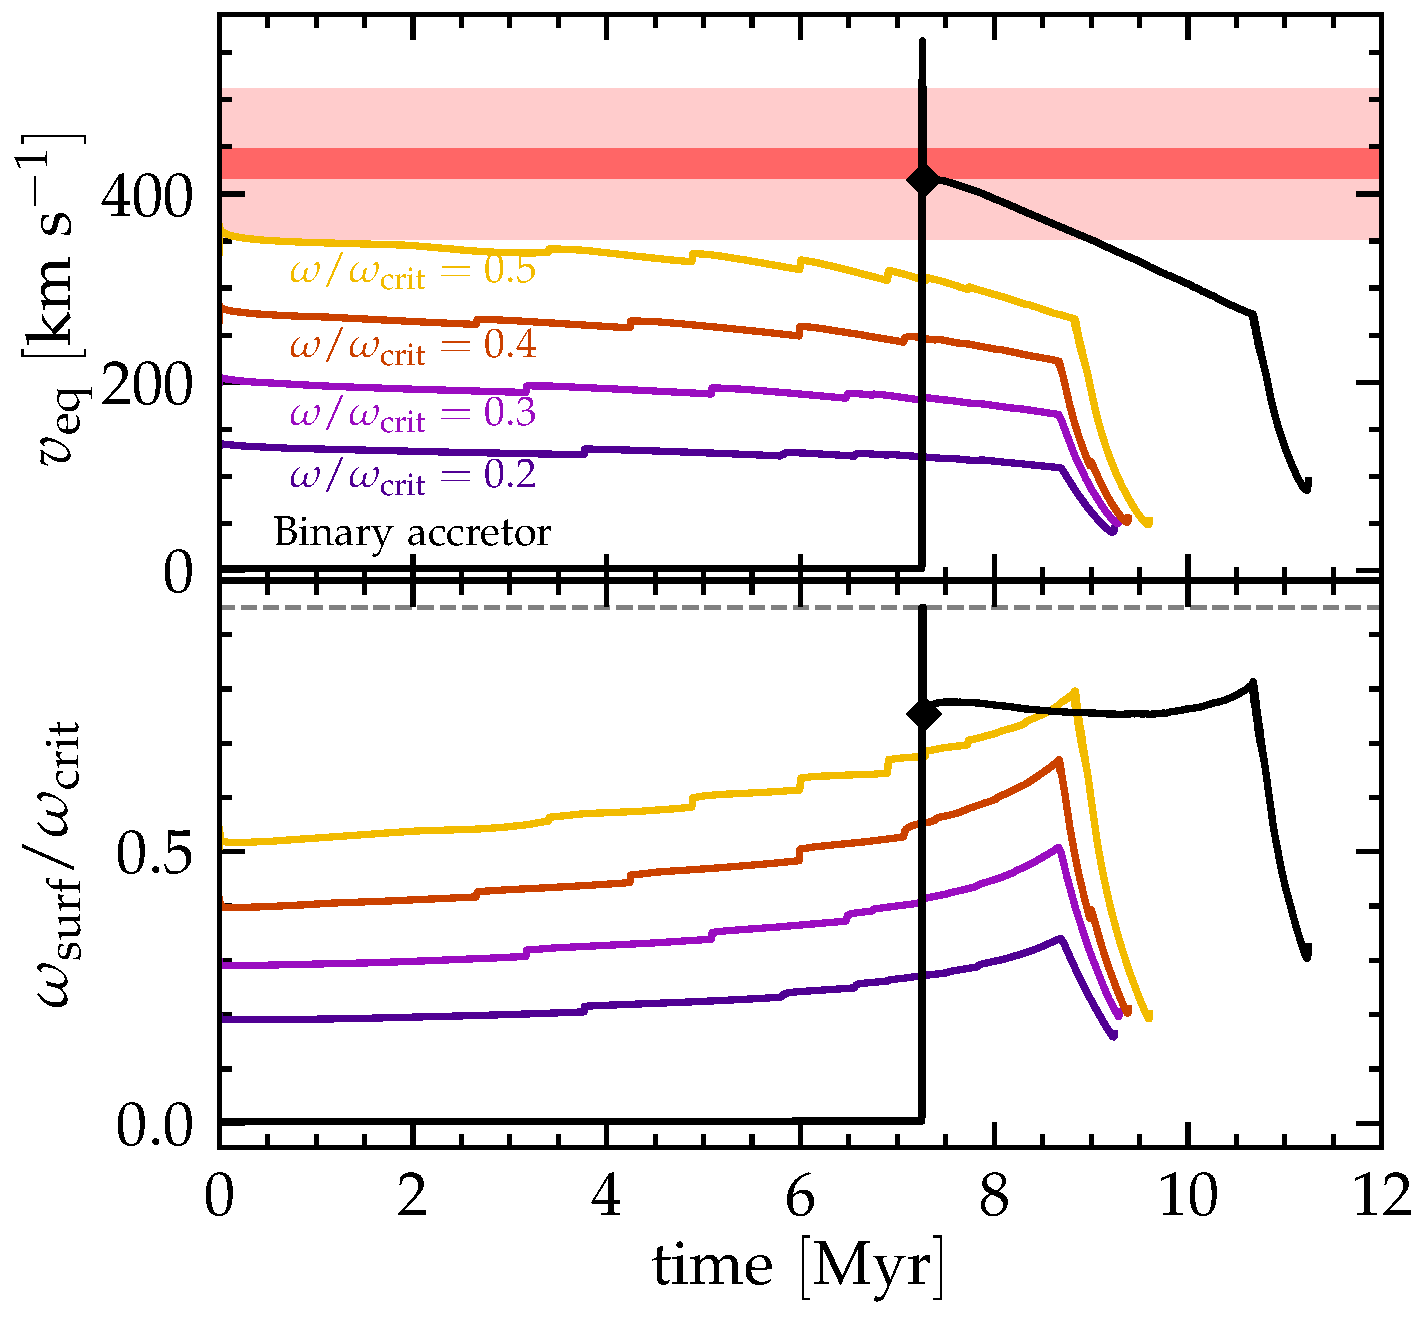
\includegraphics[width=0.5\textwidth]{zeta_rot}
  \caption{Surface averaged rotation rate for the accretor
    model. At $\sim$7.25\,Myr the mass transfer quickly spins
    up the accretor at critical rotation. By the time the donor
    detaches from the RLOF the accretor is still spinning at
    $\sim$$400\,\kms$. At this point (beginning of the dot-dashed line), we continue the evolution as a single star, and the accretor quickly spins down. Note however that we use a wind mass-loss rate from \cite{vink:01}, which is observed to be
    $\sim$2 orders of magnitude too high \citep{marcolino:09}.}
  \label{fig:surf_rot}
\end{figure}



\begin{figure*}[tbp]
  \centering
  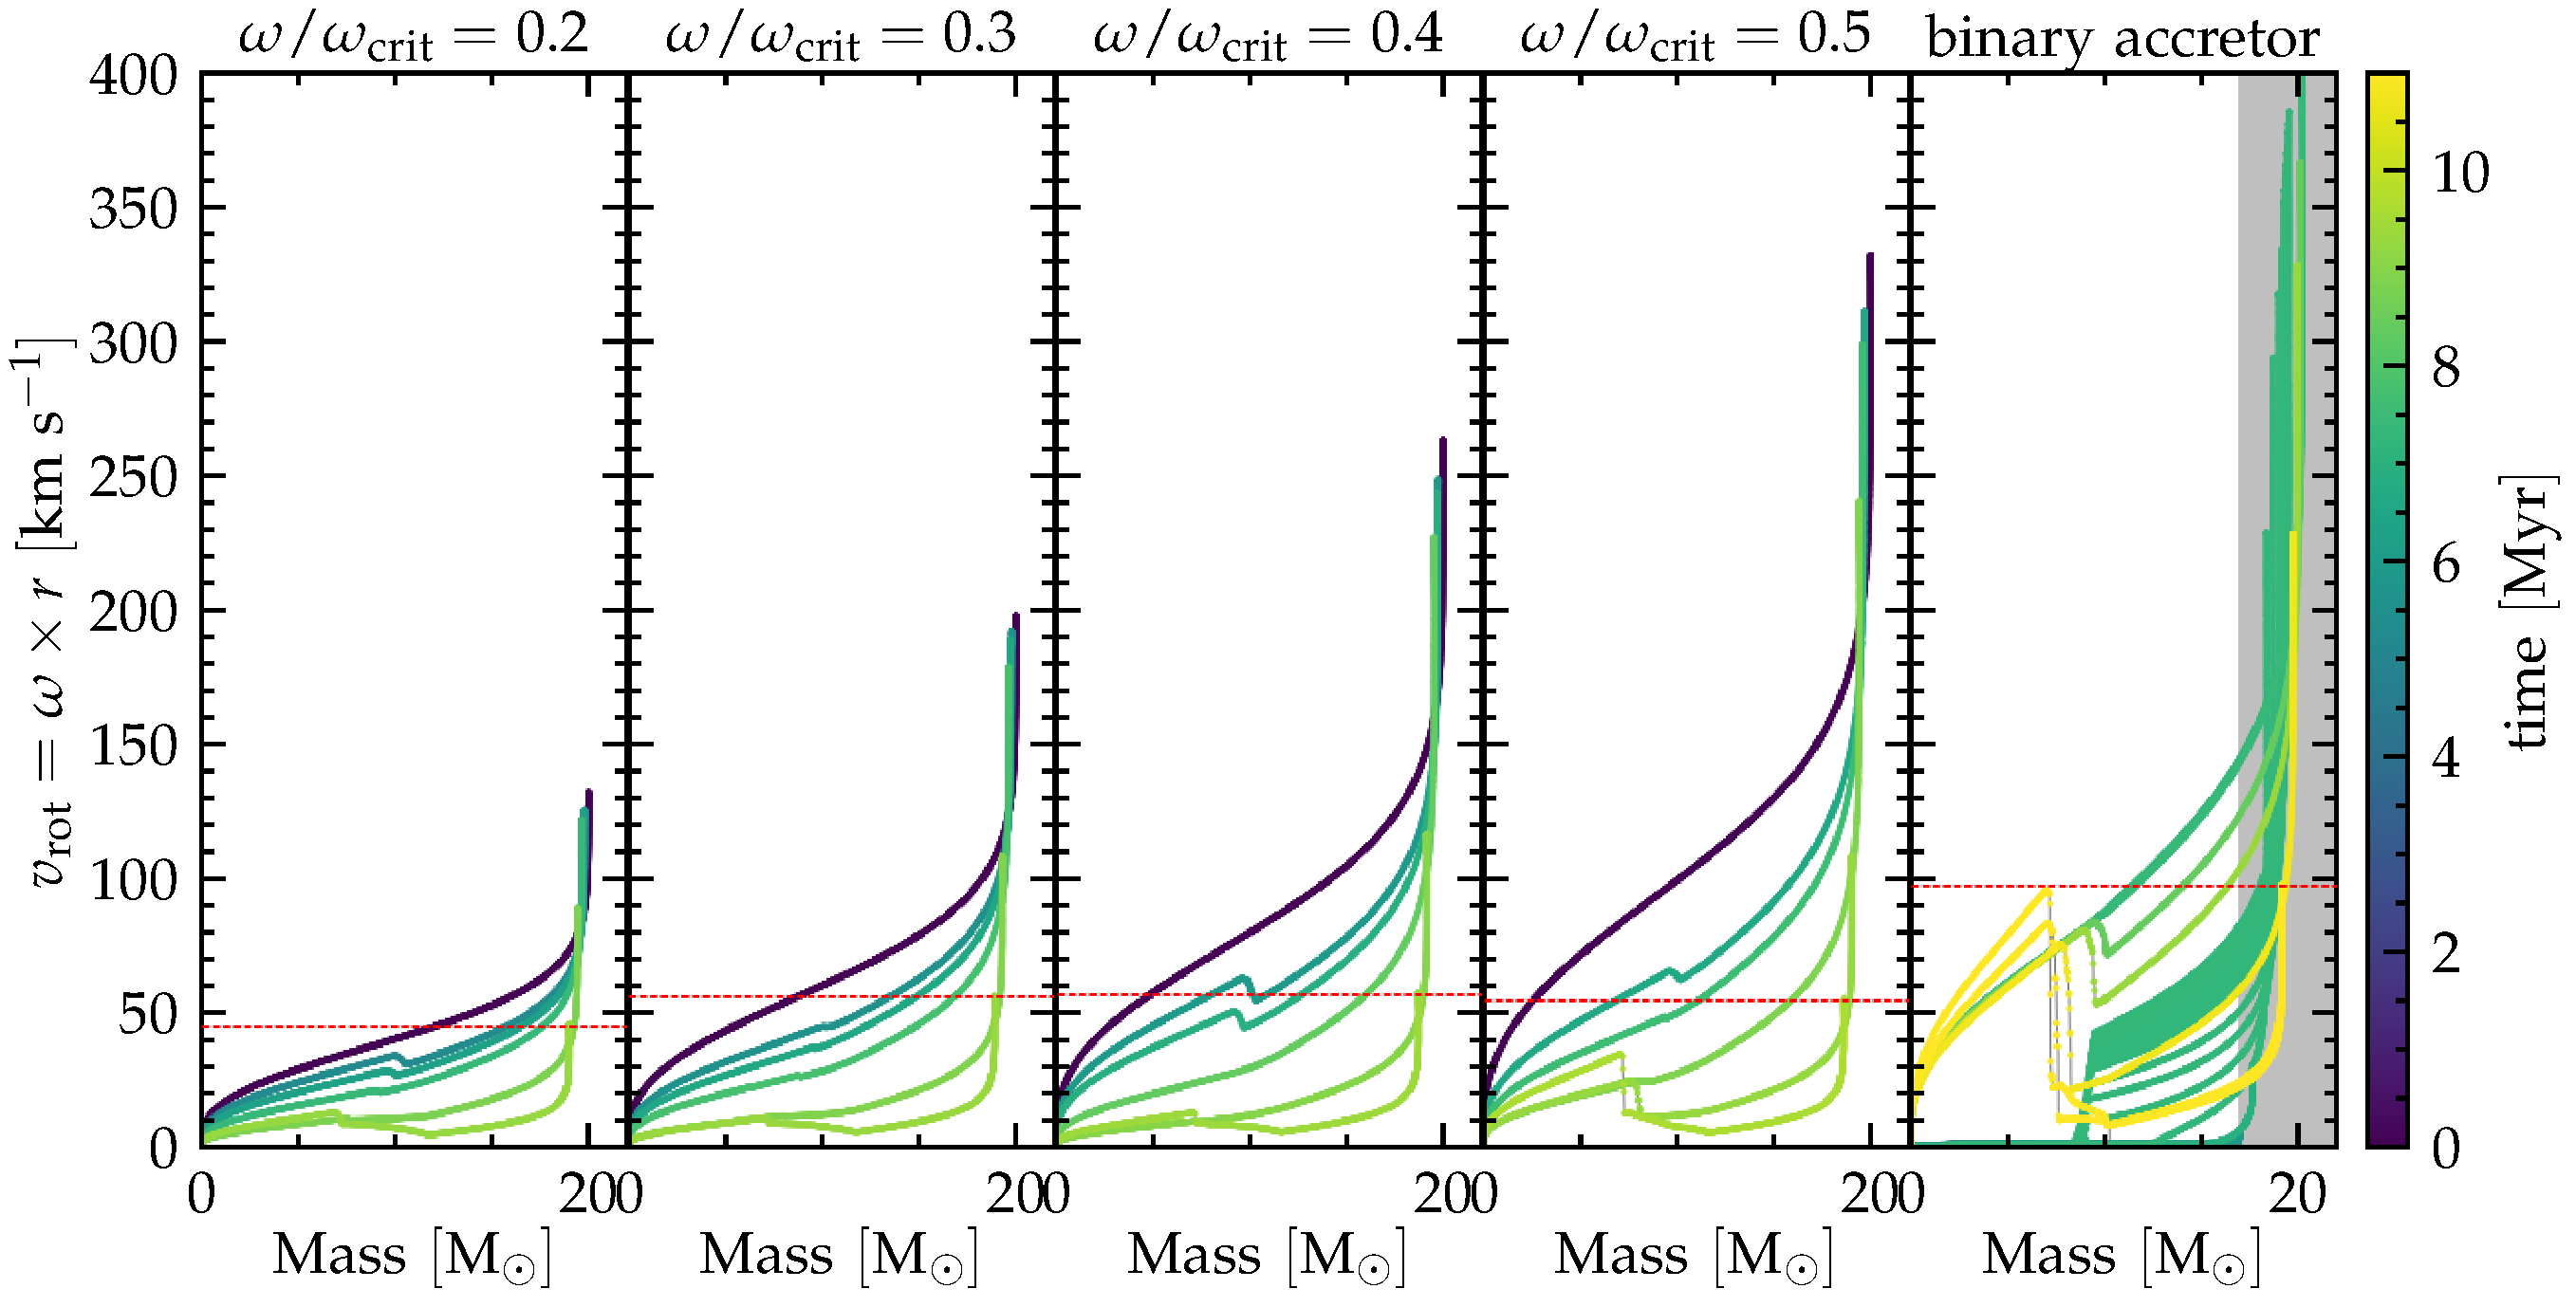
\includegraphics[width=\textwidth]{zeta_Rotational_struct}
  \caption{Internal rotational profile for $20\,M_\odot$ single star models with
    increasing $\omega/\omega_\mathrm{crit}$ at birth (first four
    panels), and for the accretor of our fiducial binary. As in
    \Figref{fig:n14}, the colors go from dark (close to ZAMS) to light
    at TAMS, and the thin dashed red line mark the TAMS surface
    rotation rate. In the last panel, the gray area indicates mass
    accreted during RLOF. The yellow lines (TAMS) in the last panel
    show that the core of the accretor is rotating almost as fast as
    its surface, and both are faster than the surface of single star
    models.}
  \label{fig:struct_rot}
\end{figure*}

One of the main distinguishing features of \zoph\ is its extremely
high surface rotation rate. Spectroscopic measurements of the
projected rotational velocity exceed $v\sin(i)\gtrsim 400\,\kms$,
which implies close to critical rotation. \cite{zehe:18} recently
estimated $v\sin(i)=432\pm16\,\kms$ and $i\sim56$ degrees. The
extremely fast rotation rate is confirmed by the centrifugal
deformation found by \cite{gordon:18}.

\Figref{fig:surf_rot} shows the surface average rotation rate of our
accretor model as a function of time (ignoring the projection angle
$i$). The dark red band corresponds to the $v\sin(i)$ from
\cite{zehe:18}, and the lighter band shows a range of 5 times their
error bar.

The initial binary is wide enough that the initial tidal
synchronization implies a very low rotation. At 7.25\,Myr, RLOF
rapidly spins up the accretor to critical rotation, up to
$v_\mathrm{crit}\simeq520\,\kms$. The star remains fast rotating
throughout the mass transfer phase, which ends at the black diamond in
\Figref{fig:surf_rot}. In the remaining evolution, the star spins down
progressively through wind mass loss, and within $\sim$2\,Myr its
averaged surface rotational velocity drops below $350\,\kms$. Close to
the end of the main sequence, the internal transport of angular
momentum causes a change in the spin-down slope.

\Figref{fig:surf_rot} shows that, without accounting for the
inclination angle, our model can retain a significant surface rotation
for a time comparable to the kinematic age of the star, which is
shorter than the remaining main-sequence lifetime. We emphasize that
throughout its evolution this model is computed using the
\cite{vink:00, vink:01} wind mass-loss rate with full efficiency. This
is two orders of magnitude higher than the wind mass loss rate
reported by \cite{marcolino:09} (however, see
\citealt{lucy:12}). While this may impact the evolution of the
binary even before RLOF, it increases the spin-down rate of
our model compared to the observations. We expect that an accreting star
modeled with lower wind-mass loss rate post-RLOF would retain an even
higher surface rotation for longer (see also \Secref{sec:single_star_uncertainties}).


\subsubsection{Comparison to single fast-rotating stars}


To illustrate the angular momentum transport in our accretor stars, it
is helpful to compare with the single rotating $20\,M_\odot$
models. The internal rotational profile of a single star rigidly rotating at
birth is different than the profile obtained spinning up the secondary
star at a later evolutionary stage and from its surface. This even within
the framework of a specific model for the angular momentum transport
in stars \citep{spruit:02}.

\Figref{fig:struct_rot} shows the internal equatorial
rotational velocity $v_\mathrm{rot}=\omega\times r$. As in
\Figref{fig:n14}, the first four panels show single rotating stars
with increasing initial $\omega/\omega_\mathrm{crit}$, the last panel
shows our accretor model, and the colors go from dark (close to zero
age main sequence, ZAMS) to light
(TAMS), with the accretor reaching lighter colors because of its
rejuvenation (see \Secref{sec:mix_comparison_single}). The gray area in the last panel represents mass accreted
during RLOF.

The thin dashed red lines in each panel mark the TAMS surface rotation
rates: all our single star models reach a TAMS surface
$v_\mathrm{rot}\simeq50\,\kms$. Initially faster rotating models spin
down more in their outer layers, have slightly longer main sequence
lifetimes (because of rotational mixing increasing the available fuel), and develop stronger differential rotation which
drives more inwards transport of angular momentum. The single star
profiles show the progressive development of a core-envelope
interface, and the core rotation rate is sensitive to the initial
value of $\omega/\omega_\mathrm{crit}$.

Conversely, the last panel shows that the entire interior of the
accretor has a negligible equatorial rotational velocity until
RLOF. Because of binary interactions, the accretor is spun up later in
its evolution, as fast as it can spin up to
$\omega/\omega_\mathrm{crit}\simeq1$, and rotation does not start as
rigid, but instead angular momentum is injected from the top. In our
model, inward transport of angular momentum creates the monotonically
increasing $v_\mathrm{rot}$ profile seen in the green lines of the
last panel. When angular momentum is transported across the chemical
gradient at the edge of the convective core, a discontinuity stronger
than in the single stars arises.

By the end of the main-sequence evolution of the accretor, the surface
still spins with $v_\mathrm{rot}\simeq100\,\kms$ (twice as fast as the
single star models). Perhaps more importantly, the outer-edge of the
core has a similar rotational velocity as the surface, and much larger
than the rotational velocity of the single star models. The fact that
the accretor is spun-up late in its main-sequence evolution, to
critical rotation, and from the top (instead of starting from rigid
rotation) leads to faster spinning cores than fast rotating single
stars. This might have important implications for the explosion of the
initially less massive star and the rotation rate of
the resulting compact objects, and the analysis of compact object
spins from gravitational-wave events \citep[e.g.,][]{zaldarriaga:18, qin:18, callister:21}.

\section{Robustness of the models and discussion}
\label{sec:discussion}

Models of the interior evolution of stars require the choice of
several poorly constrained parameters, the majority arising from the
one-dimensional representation of multi-dimensional phenomena
(convection, mixing, rotation, etc.). This remains true when modeling
two stars in a binary, with the added caveat that even more free
parameters enter in the treatment of binary interactions (and in
particular mass transfer). In \Secref{sec:single_star_uncertainties}
We report on exploration of parameter variations for each individual
star. We discuss parameters governing the mass transfer phase in
\Secref{sec:bin_param}, the initial binary architecture in
\Secref{sec:bin_init}, and the consequences of the assumed SN
explosion of the companion in \Secref{sec:SN_comp}.


\subsection{Uncertainties in the single-star physics}
\label{sec:single_star_uncertainties}

For our model of \Secref{sec:best_model}, we have assumed an initial
metallicity $Z=0.01$ informed by the asteroseismology of low mass
stars in the parent association Upper-Centaurus-Lupus \citep[e.g.,][]{murphy:21}. Moreover,
we have assumed that mass fractions of each element scale with the Solar values
\citep{grevesse:98}, which might not be appropriate especially for
massive stars \citep[e.g.,][]{grasha:21}. With these assumptions, the
initial mass fraction of $^{12}\mathrm{C}$ and $^{14}\mathrm{N}$ are
lower than the observed values for \zoph. Even though their values at
the surface of the accretor increase during mass transfer, our model
still slightly under-predicts them. Improved agreement could be
obtained changing the ratio of abundances to non-solar values, or by
changing the efficiency of downward rotational and thermohaline mixing
which dilutes the accreted material into the secondary's envelope.

We also run a model identical to the one described in
\Secref{sec:best_model}, except with $Z=Z_\odot=0.0142$
\citep{asplund:09}. Qualitatively, the binary evolution remains
similar, with the higher metallicity stars having slightly larger
radii and cooler $T_\mathrm{eff}$ at a given luminosity. This still
produces a stable case B RLOF, however, the accretor track is
displaced on the right on the HRD. Thus, matching the high present-day
$T_\mathrm{eff}=32\,000\pm2\,000$ of \zoph\ (e.g., \citetalias{villamariz:05}) requires more
massive and hotter accretors (see also \Secref{sec:bin_init}).

Rotation is a critical ingredient of our models: it governs the
equatorial radius extent and thus the $\omega/\omega_\mathrm{crit}$
and mass transfer efficiency (see \Secref{sec:bin_param}), through
Eddington-Sweet meridional circulations it determines outward mixing
from the core, and more importantly inward mixing from the surface.
We emphasize that the shellular approximation used in one-dimensional
stellar evolution codes might not be appropriate for
$\omega/\omega_\mathrm{crit}\simeq 1$ reached by our accretor star
during RLOF. Decreasing by a factor of 10 the diffusion coefficient
for Eddington-Sweet meridional circulations has a very small effect on
the HRD evolution of the accretor. However, the noisiness during the
late RLOF phase (for $T_\mathrm{eff}\gtrsim10^{4.5}$\,K in
\Figref{fig:HRD_both}) increases in amplitude slightly, confirming
that the details of this part of the evolution are sensitive to the
treatment of rotational mixing. We were unable to run models turning
completely off Eddington-Sweet meridional circulations past the
``v-shaped'' feature in \Figref{fig:HRD_both}.

Our models assume a Spruit-Tayler dynamo \citep{spruit:02} for the
transport of angular momentum throughout the evolution. Adopting the
stronger angular momentum transport from \cite{fuller:19} might result
in a more efficient spin-down of the surface during RLOF, possibly
allowing for more accretion of mass. Moreover, this might enhance the
differences between the internal rotational profile of single
fast-rotating stars and accretors in binaries.

Similarly, during RLOF, thermohaline mixing in the envelope becomes
important. We have explored models enhancing the efficiency of this
mixing process by a factor of 100, however, this caused our models to
crash during RLOF after the ``v-shaped'' feature corresponding to the
accretion of nuclearly processed material.

Finally, to address the ``weak wind problem'', we also attempted
running models with artificially decreased wind mass loss rate
\citep[e.g.,][]{renzo:17}, but these resulted in super-critical
$\omega/\omega_\mathrm{crit}>1$ accretor stars with untrustworthy
numerical results.

While the number of free parameters resulting in a successful
computation is rather limited, we emphasize that this remains often
true for calculation of single massive star evolution.

\subsection{Uncertainties in the treatment of mass transfer}
\label{sec:bin_param}

We regulate the accretion efficiency through the rotational
enhancement of mass loss \citep[e.g.,][]{langer:98}.
However, whether critical rotation can effectively stop the accretion
of matter is unclear. \cite{popham:91} and \cite{paczynski:91}
argued that accretion of mass (but no angular momentum) might be
possible even at or beyond critical rotation.

During RLOF, the total amount of mass lost by the donor is
$\Delta M_\mathrm{donor} \simeq 10.6\,M_\odot$, of which only
$\Delta M_\mathrm{accretor}\simeq 3.4\,M_\odot$ are successfully
accreted. This corresponds to an overall mass transfer efficiency
$\beta_\mathrm{RLOF}\equiv |\Delta M_\mathrm{accretor}|/|\Delta M_\mathrm{donor}| \simeq 0.3$,
although the accretion efficiency is \emph{not} constant throughout
the mass transfer \citep[e.g.,][]{vanrensbergen:06}. In our models,
the mass transfer efficiency depends on the radial and rotational
evolution of the accreting star. During RLOF, the accretor is out of
gravothermal equilibrium with significant impact on its radius and
ultimately on the amount of mass transferred and its angular
momentum. In reality, the gas stream between the two stars, the
formation of a disk, and the geometric distorsion of the outer layers because
of the centrifugal forces would not follow the spherical symmetry
imposed by 1D codes such as \texttt{MESA}.

While the mass transfer efficiency $\beta_\mathrm{RLOF}$ and
importantly its time-evolution need further attention, we emphasize that most studies, especially
using rapid population synthesis tools, typically assume a
constant $\beta_\mathrm{RLOF}$ and neglect to model the
out-of-equilibrium phase of the accretor and how this can impact the
binary and orbital evolution.

Another free parameter in the treatment of mass transfer is the
specific angular momentum of the accreted material. In our models, for
the sake of numerical stability, we assume the incoming material and
the stellar surface to have the same specific angular momentum. This
approximation corresponds to a scenario where angular momentum
transport in the circumstellar disk during RLOF quickly homogenizes
the rotation rate and provides a relatively slow spin-up of the
accretor star.

We also attempted calculations using the algorithm from
\cite{demink:13} based on the fit from \cite{ulrich:76} to the
numerical results of \cite{lubow:75}. This algorithm distinguishes between
direct impact of the L1 stream and circumstellar disk
formation and determines the specific angular momentum of the incoming
material. However, these models proved numerically more unstable and
providing less trustworthy results. Generally speaking, allowing for a
faster accretion of angular momentum results in less radial expansion
of the accretor (cf.~\Figref{fig:HRD_both}), faster spin-up, and a lower overall mass
transfer efficiency $\beta_\mathrm{RLOF}$.

Finally, while the composition of the transferred material is
determined by the structure of the donor and the mass transfer rate
calculated following \cite{kolb:90}, we still need to specify its
specific entropy when it reaches the accretor surface. We follow the
common practice of assuming the specific entropy of the incoming
material to be same as the accreting surface. The scenario justifying
this hypothesis is that during RLOF the matter is
sufficiently optically thin so radiative processes can rapidly
equalize the entropy between the RLOF stream and the accreting
surface. However, the very large mass-transfer rates we find
(cf.~\Figref{fig:MT}) might result in optically thick flows for which
this approximation might not be appropriate.

\subsection{Variations in the initial binary parameters}
\label{sec:bin_init}

The initial donor mass $M_1$, mass ratio $q=M_2/M_1$, and the period of the progenitor binary of \zoph\ cannot be directly
constrained from observations. We have explored variation in these values, and the
qualitative behavior of the models is similar.

Shorter initial periods results in larger post-RLOF orbital
velocities, and thus larger runaway velocities if the binary is
disrupted at the first SN (see \Secref{sec:SN_comp}). For example, taking $P$=75\,days
(cf.~100\,days in our fiducial model in \Secref{sec:best_model}), the
binary still experiences stable case B mass transfer, but the
post-RLOF orbital velocity of the accretor is about $60\,\kms$, that
is $\sim$$10\,\kms$ higher
than in our fiducial model.

Increasing the donor mass also has a similar effect on the post-RLOF orbital velocity of the accretor. Using
$M_1=30\,M_\odot$ (cf.
$25\,M_\odot$ in \Secref{sec:best_model}),
$M_2=17\,M_\odot$, and
$P$=100\,days, we obtain a post-RLOF velocity of
$65\,\kms$. However, this produces a stripped donor of
$\sim$16\,$M_\odot$ at RLOF detachment, with stronger wind mass loss. Therefore this binary is expected to widen relatively more than our fiducial model of \Secref{sec:best_model}, slowing down the secondary. The increased mass of the stripped star could also imply a lower chance of exploding for the donor (however, see \Secref{sec:SN_comp}).

The higher $M_1$ does not significantly change the post-RLOF total
mass of the accretor, with $M_2$ remaining about $\sim$20.5\,$M_\odot$, since
in our models accretion is regulated mostly by the spin up of the
accretor, and we do not couple the specific angular momentum of the transferred
material to the orbit or the donor's spin.

However, changing the initial mass ratio also changes the difference
between the main-sequence lifetime of the two stars, and thus how far
along the main sequence the accretor is at the onset of RLOF. The observed
position of \zoph\ on the HRD, particularly its relatively high
$T_\mathrm{eff}$ are difficult to reproduce assuming initially less
massive accretors (which would remain too cool even after accreting
mass), or more equal initial mass ratio (which would produce a too
evolved accretor at the onset of mass transfer).

\subsection{The explosion of the former companion}
\label{sec:SN_comp}

Throughout this study, we have assumed the ``binary SN scenario'' to
explain the runaway nature of \zoph:
after the mass transfer phase, the explosion of the donor breaks the
binary and ejects the accretor at roughly its pre-explosion orbital
velocity \citep[e.g.,][]{renzo:19walk}. This fate occurs to the
majority of massive binary systems, and \zoph\ might be the best
example of it \citep[e.g.,][]{blaauw:52, blaauw:61,
  hoogerwerf:00}. \cite{neuhauser:20} suggested not only the companion
successfully exploded producing the pulsar PSR B1706-16, but that the
explosion produced radioactive $^{60}\mathrm{Fe}$ which polluted
Earth.

From kinematic and orbital considerations they estimated the pulsar
received a natal kick of
$253\pm54\,\kms$, which would be sufficiently large to unbind the binary \citep{kalogera:96, tauris:15}.  The ejecta mass would depend on the post-RLOF wind mass loss of our donor star, which we do not model.  At the end of our binary model (black diamond in \Figref{fig:HRD_both}), our stripped donor is
$\sim$$9.4\,M_\odot$, with a surface H fraction of $X\lesssim0.2$ for
a layer of $\Delta M \simeq 2.5\,M_\odot$.  Its wind mass-loss rate is
$\sim10^{-5}\,M_\odot \ \mathrm{yr^{-1}}$ (cf.~\Figref{fig:MT}),
likely to increase as it contracts into a Wolf-Rayet star and
increases its luminosity and effective temperature. We expect its
explosion to appear as H-less type Ib SN. Although our stripped donor
is rather massive, recent studies hints at a higher ``explodability''
of donor stars in binary systems \citep[e.g.,][]{schneider:21,
  laplace:21, vartanyan:21}.

We have neglected the impact of the explosion on the structure of the
accretor star. At the time of the explosion, the accretor subtends a
solid angle $\sim$$R^2/a^2\simeq
0.05$\,degrees with $R$ the accretor radius and
$a$ the binary separation. We neglect the post-RLOF wind-driven orbital widening for this estimate.  The blast wave will hit the accretor causing mass loss -- directly via ablation and by injecting energy in the envelope, inflating it and enhancing its wind \citep{wheeler:75, tauris:98, podsiadlowski:03, hirai:18}.  Because of the SN shock, the just ejected new runaway star might appear bloated and redder (long before it overtakes the slowing SN remnant). The impact of this brief out of thermal equilibrium phase on the stellar spin should be investigated further.

Using 2D hydrodynamic simulations of the star-SN ejecta interactions in close binaries ($a\lesssim
60\,R_\odot$, cf. $a\gtrsim
343\,R_\odot$ in our fiducial binary model), \cite{hirai:18} found that the companion star recovers its pre-explosion luminosity and effective temperature within a few years to decades, and the amount of mass removed by the SN shock is
$\lesssim10^{-2}\,M_\odot$.  The SN ejecta might also pollute the surface of the runaway depositing processed nuclear material \citep[e.g.,][]{przybilla:08}. However, enhahnced mass loss, rapid rotation and mixing might quickly dilute the yields.


\section{Conclusions}
\label{sec:conclusions}

We presented self-consistent 1D calculations of coupled stellar models
with masses $\gtrsim 20\,M_\odot$ with the \texttt{MESA} binary stellar
evolution code. As a first application, we focused on finding a
model for \zoph, assuming its runaway nature is explained by the
binary SN scenario.

We found that it is possible to explain the observed features of
\zoph\ with a relatively wide and massive binary initialized with
$M_1=25\,M_\odot$, $M_2=17\,M_\odot$, and $P=100$\,days at metallicity
$Z=0.01$ (see \Secref{sec:best_model}). This binary system experiences dynamically-stable Roche
lobe overflow after the end of the main sequence of the initially more massive star
(case B). Standard stellar physics assumptions for modeling rotation,
mixing, and mass transfer in binaries reproduce reasonably well the
main features of \zoph\ (see \Secref{sec:methods} and Appendix~\ref{sec:software}). Specifically,
$\sim$$1.5-2$\,Myrs after the end of mass transfer, corresponding to the
remaining donor's lifetime at the end of our simulations plus the kinematic age of \zoph,
the accretor star in our model has the following quantities in the correct ballpark:
\begin{itemize}
\item Luminosity and effective temperature;
\item Total mass;
\item Runaway space velocity;
\item Fast surface rotation (albeit possibly on the low side, cf.~weak wind problem);
\item enhanced $^4\mathrm{He}$ and $
  ^{14}\mathrm{N}$ surface mass fraction;
\item small variations in $^{12}\mathrm{C}$ and $^{16}\mathrm{O}$ surface mass fractions.
\end{itemize}

We emphasize that the surface composition alone would not be a smoking-gun,
especially given the large uncertainties in the treatment of rotation
and mixing in stellar evolution models. However, alternative scenarios where \zoph\
evolved as a single fast-rotating star require ad-hoc explanations for the runaway velocity,
and have been shown by \citetalias{villamariz:05} to struggle in reproducing
surface mass fractions, apparent age, mass, and rotation rate simultaneously.

%  in terms of its spatial velocity, its surface
% $^{14}\mathrm{N}$ and $^4\mathrm{He}$ enhancement, its rotation rate,
% age and position on the Hertzsprung-Russell diagram.

In contrast with \cite{vanrensbergen:96}, in our model the
$^{14}\mathrm{N}$ and $^4\mathrm{He}$ rich surface composition is not
the result of pure outward rotational mixing.  Instead, this material
is transferred from the receeding core of the donor star and mixed
from the surface inwards by rotation and, to a smaller degree, by
thermohaline mixing.  Thus, the present day surface mass fractions of
\zoph\ put a coupled constrain the mass transfer efficiency and mixing
in the accretor. Therefore, such star should \emph{not} be used to
calibrate models of rotational mixing in single star evolution, nor
its more extreme version of chemically homogeneous evolution.

The spin up of the accreting star occurs late in its evolution
($t\gtrsim7.25$\,Myr for our fiducial binary) and
reaches to critical surface rotation
$\omega/\omega_\mathrm{crit}\simeq 1$. % This allows the accretor star
% to be simultaneously nitrogen rich and still fast rotating after the
% mass transfer phase.
The treatment of close-to-critical rotation
impacts the accretion efficiency, the radius evolution, and the inward
mixing.

An important difference we find between our accretor model and
comparable fast-rotating single star models is their internal rotation
profile. Single-stars rotating rapidly from birth are initialized as
rigid rotators, and spin down significantly both at the surface and
inside. Conversely, in our accretor models angular momentum is
injected late and from the top. When this angular momentum is
transported into the core by the Spruit-Tayler dynamo, it results in a
much faster rotating helium core, with potential implications for the
final explosion and the resulting compact object born from the
accretor star in an interacting binary system. %  We emphasize that our models assume a
% Spruit-Tayler dynamo \citep{spruit:02} for the transport of angular
% momentum. Recently, \cite{fuller:19} proposed a stronger angular
% momentum transport which would presumably result in a faster spin down
% of the surface (possibly allowing for more accretion during mass
% transfer) and even more significant core spin-up in our accretor.


We also consider variations in the initial parameters and in the
implementation of physical processes, discussed in
\Secref{sec:discussion}.  Less massive secondaries remain too cool
throughout the evolution to be compatible with \zoph, and more equal
initial mass ratios lead to a more evolved accretor at the onset of
mass-transfer, again resulting in too cool temperatures.

Improving our understanding of the evolution of the initially less
massive stars in massive binary systems is crucial for the upcoming
large surveys (astrometric, photometric, time-domain and
spectroscopic) and for the understanding of the evolution of
gravitational-wave progenitors in isolated binaries. Although
presently single, the nearest O-type star to Earth, \zoph, can be used
as an anchor point for the modeling of accretors. Our models
demonstrate that a broad agreement with observations can be
achieved with standard stellar evolution assumptions. Future efforts
should extend these models to a wider mass, period, mass ratio, and metallicity
range to investigate the impact of binary evolution on the life,
explosion, and after-life of the secondary stars in massive binary
systems.

\software{
  \texttt{mesaPlot} \citep{mesaplot},
  \texttt{mesaSDK} \citep{mesasdk},
  \texttt{ipython/jupyter} \citep{ipython},
  \texttt{matplotlib} \citep{matplotlib},
  \texttt{NumPy} \citep{numpy},
  \MESA \citep{paxton:11,paxton:13,paxton:15,paxton:18,paxton:19}
}

\acknowledgements{We are grateful to E.~Zapartas, A.~Jermyn,
  M.~Cantiello, and R.~Neuh\"auser for helpful discussions.}

\appendix

\section{\texttt{MESA} setup}
\label{sec:software}

% \todo{MLT--?}

We use \code{MESA} version 15140 to compute our models.  The
\code{MESA} equation of state (EOS) is a blend of the OPAL \citet{Rogers2002}, SCVH
\citet{Saumon1995}, PTEH \citet{Pols1995}, HELM \citet{Timmes2000},
and PC \citet{Potekhin2010} EOSes.

OPAL \citep{Iglesias1993, Iglesias1996} provides the main radiative
opacities, with low-temperature data from \citet{Ferguson2005} and the
high-temperature from \citet{Buchler1976}. Electron conduction
opacities are from \citet{Cassisi2007}.

Nuclear reaction rates are a combination of rates from NACRE
\citep{Angulo1999}, JINA REACLIB \citep{Cyburt2010}, plus additional
tabulated weak reaction rates \citet{Fuller1985, Oda1994,
  Langanke2000}. Screening is included via the prescription of
\citet{Chugunov2007}.  Thermal neutrino loss rates are from
\citet{Itoh1996}. We use a
22-isotope nuclear network (\texttt{approx\_21\_plus\_cr56}).

The inlists, processing scripts, and model output will be made available at~\url{10.5281/zenodo.4701565}.

\section{Internal composition profile evolution}
\label{sec:X_fig}


\Figref{fig:composition_huge} compares the internal evolution of the composition
profile of single rotating stars with our accretor model.
We show mass fractions of $^{12}\mathrm{C}$  and $^{16}\mathrm{O}$ to complement the
mass fraction of $^{14}\mathrm{N}$ shown in \Figref{fig:n14}, and
reproduced also in the middle panel of \Figref{fig:composition_huge}.


\begin{figure*}[hp]
  \centering
  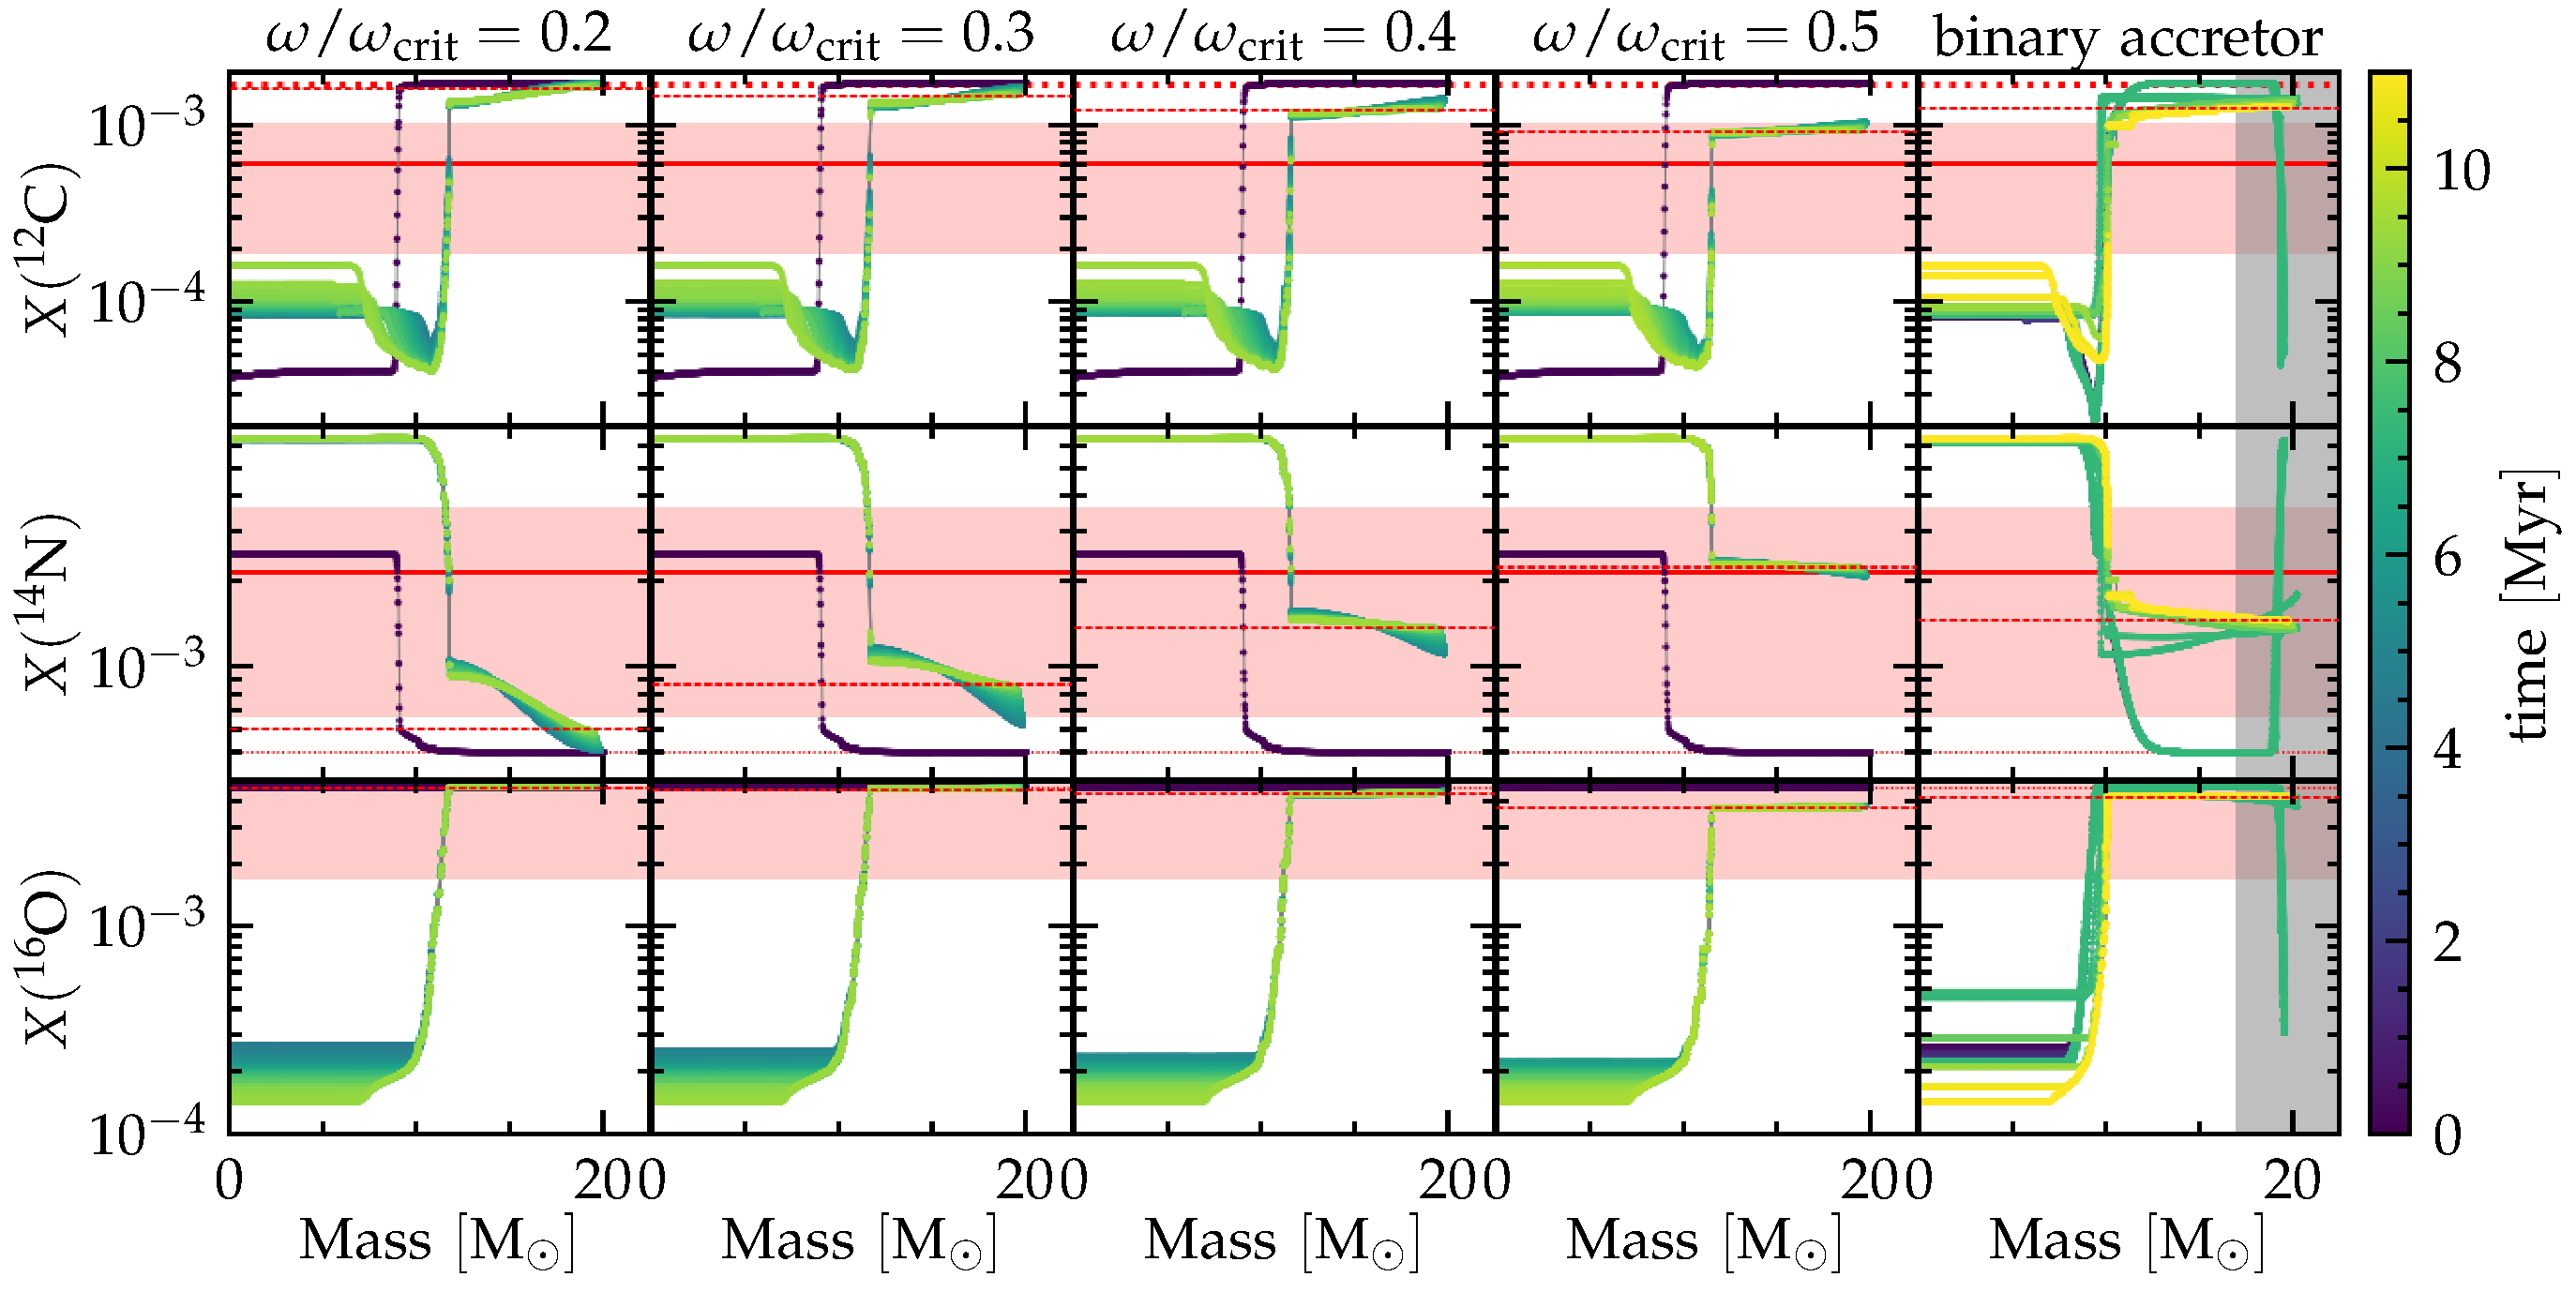
\includegraphics[width=\textwidth]{huge_composition}
  \caption{Same as \Figref{fig:n14}, but for $^{12}\mathrm{C}$ (top
    panel), and $^{16}\mathrm{O}$ (bottom panel). The first four
    panels show single rotating stars of initially $20\,M_\odot$, the
    rightmost panel shows the accretor in our fiducial binary. The middle panel is
    exactly the same as \Figref{fig:n14}. Thick red dotted lines mark the
    initial mass fractions, thin red dashed lines the TAMS surface mass
    fraction, the solid red lines and the semi-transparent red bands
    correspond to the values inferred by \citetalias{villamariz:05}
    using the surface H mass fraction from our model. The tracks go
    from dark (roughly corresponding to ZAMS) to light colors, with the
    lightest color corresponds to TAMS.}
  \label{fig:composition_huge}
\end{figure*}

\section{Resolution tests}
\label{sec:res_tests}


\begin{figure*}[hp]
  \centering
  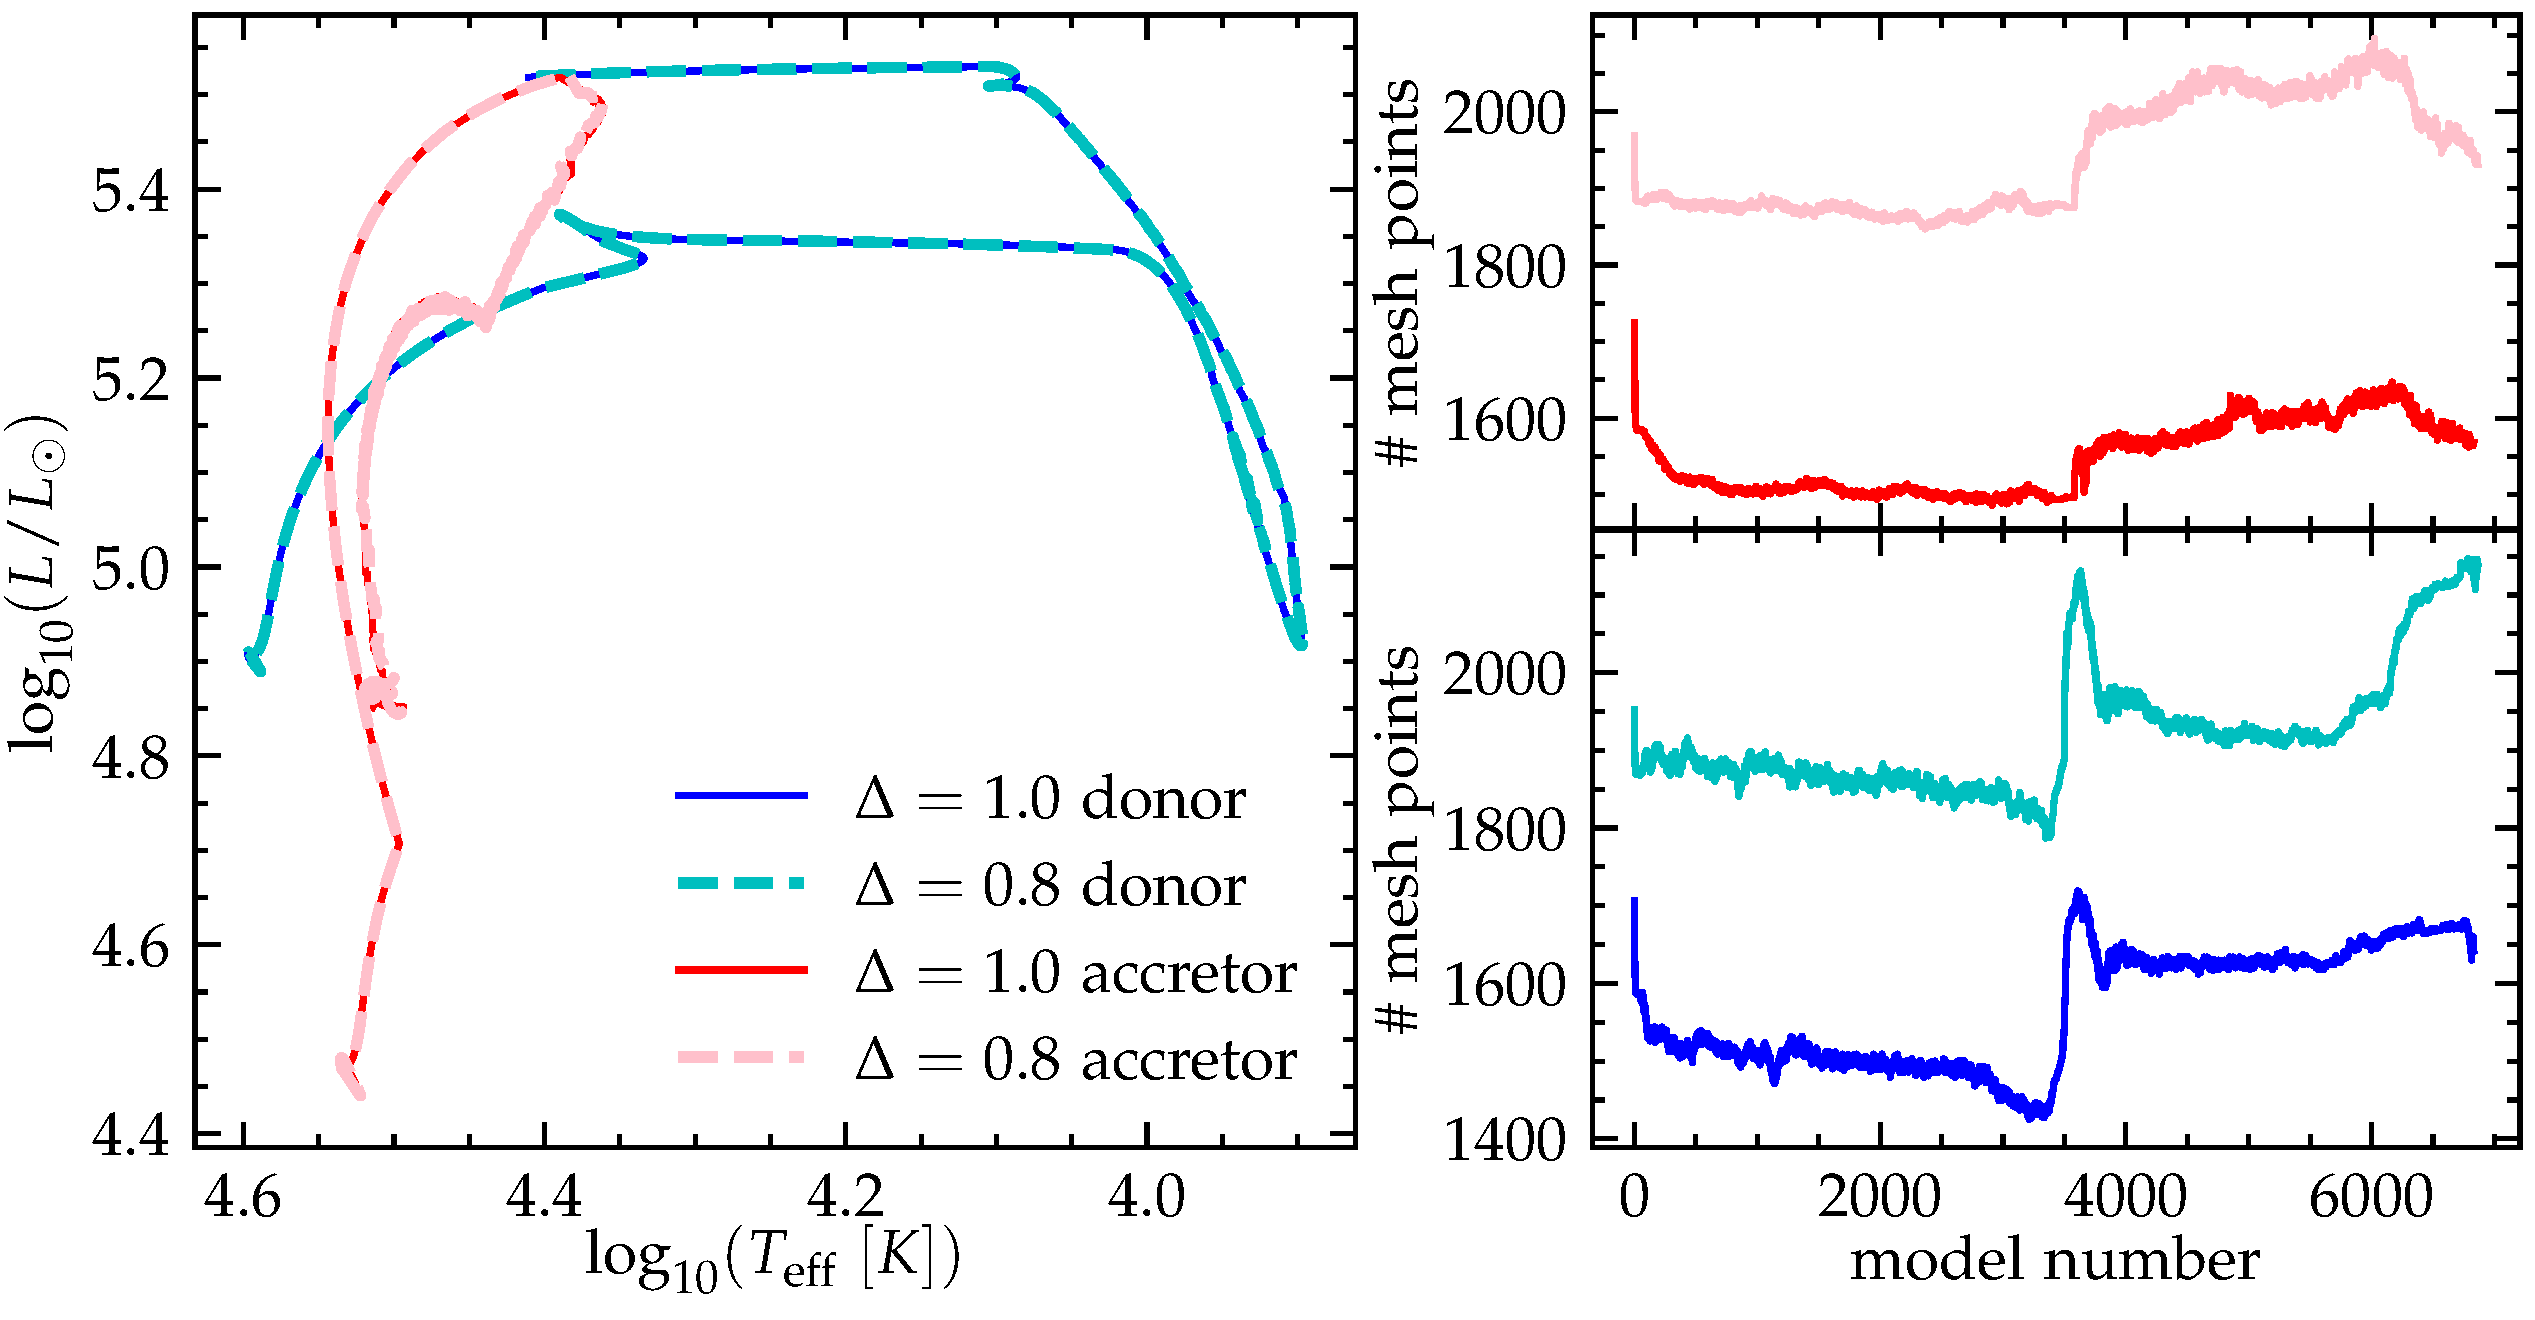
\includegraphics[width=\textwidth]{spatial_res_plot}
  \caption{Left: HRD comparison for our fiducial binary model varying
  the number of mesh points. We only show the evolution until our definition
  of RLOF detachment. Right: number of mesh points as a
  function of timestep number. In both panels, the blue/cyan tracks show the donor stars, the
red/pink tracks show the accretor. Thicker dashed lines correspond to
the models at higher resolution (i.e., lower $\Delta$ which indicates
the value of \texttt{mesh\_delta\_coeff}).}
\label{fig:sp_test}
\end{figure*}



We extensively check the numerical convergence of our stellar
evolution calculations with increasing number of mesh
points. \Figref{fig:sp_test} shows that all the features described
extensively here do not vary when increasing the spatial resolution by
decreasing \texttt{mesh\_delta\_coeff}. The right panel shows the
number of mesh points for the accretor (top) and donor (bottom) as a
function of the model number (akin to an arbitrary time
coordinate). About $\sim$7000 \texttt{MESA} models are used to compute
the binary evolution. The higher resolution run has $\sim 20\%$ more
mesh points. The left panel shows the HRD evolution until the
detachment of the binary for the two accretor models (pink/red) and
the two donor models (blue/cyan).

Similarly, we tested the numerical convergence with decreasing
timestep size. This can be done decreasing the parameter
\texttt{mesh\_time\_coeff}. However, we were unable to successfully
compute models at higher temporal resolution. Partial results show a
good agreement with our fiducial model until \texttt{MESA} becomes
unable to find a satisfying numerical solution to the stellar
structure equations (typically
during RLOF). Lower temporal resolution models showed a similar
qualitative agreement but increased noisiness during the late RLOF
phase. For our fiducial model the adaptive timestep size never exceeds
$10^{3.8}$\,years with typical pre-RLOF timesteps of the order of $10^{3.2}$\,years
and sub-decade during RLOF. The main factor limiting the timestep
sizes is the change of surface angular momentum in both stars during
the mass transfer.


\newpage
\bibliographystyle{aasjournal}
\bibliography{./zeta_ophiuchi.bib}

\end{document}

%%% Local Variables:
%%% mode: latex
%%% TeX-master: t
%%% End:
